\documentclass[a4paper,10.5pt]{report}

\usepackage[toc]{appendix}
\renewcommand{\appendixname}{Annexos}
\renewcommand{\appendixtocname}{Annexos}
\renewcommand{\appendixpagename}{Annexos}
\usepackage[catalan]{babel}
\usepackage{booktabs}
\usepackage[nottoc]{tocbibind}
\usepackage{listings}
\lstdefinestyle{mystyle}{
	language=Python,                 % Lenguaje del código
	frame=single,                    % Marco alrededor del código
	basicstyle=\ttfamily\footnotesize, % Fuente del código
	keywordstyle=\color{blue},       % Color para palabras clave (def, if, else...)
	commentstyle=\color{gray},       % Color para comentarios
	stringstyle=\color{teal},        % Color para strings
	numbers=left,                    % Numeración de líneas
	numberstyle=\tiny\color{gray},   % Estilo de los números de línea
	stepnumber=1,                     % Cada cuántas líneas numerar
	showspaces=false,                 % No mostrar espacios en blanco
	showstringspaces=false,            % No mostrar espacios en strings
	breaklines=true,                   % Romper líneas largas automáticamente
	tabsize=4,                         % Tamaño de tabulación
	captionpos=b,                      % Posición de la caption (arriba o abajo)
	morekeywords={self, as, in},       % Palabras clave adicionales
}
\lstset{style=mystyle} % Aplicar este estilo a todos los listados
\usepackage{tcolorbox}
\usepackage{parskip}
\usepackage{multirow}
\usepackage{graphicx}
\usepackage{booktabs}
\usepackage{caption}
\captionsetup{labelfont=bf}
\usepackage{hyperref}
\usepackage[arrowdel]{physics}
\usepackage[left=1.95cm, right=1.95cm, top=20mm, bottom=20mm]{geometry} 
\usepackage{fancyhdr}
\usepackage{braket}
\usepackage{amsmath, amssymb, amsfonts}
\usepackage{subcaption}
\usepackage{cancel}
\usepackage{float}
\usepackage{titling}
\usepackage{etoolbox}
\renewcommand{\labelenumi}{\textbf{\theenumi.}} 

%Definim el següent entorn per tal de poder posar abstracts a cada capítol.
\newenvironment{chapterabstract}{
	\begin{center}
		\bfseries Abstract
	\end{center}
	\quotation
}{\endquotation}

\usepackage{titlesec}
\usepackage{tikz}


\titleformat{\chapter}[display]{\normalfont\huge\bfseries}{Pràctica \thechapter}{0pt}{\vspace{0.2cm}\huge\bfseries\raggedright}

\title{\textbf{\huge{Informes de Pràctiques. \\ \vspace{0.2cm} Laboratori d'Electromagnetisme}}}
\author{Grup A1}
\date{\today}

\begin{document}
	
\begin{titlepage}
	\centering
	{\LARGE Laboratori d'Electromagnetisme \par}
	\vspace{2cm}
	{\Huge \textbf{Informes de Pràctiques} \par}
	\vspace{3cm}
	{\Large Grup A1 \par}
	\vspace{0.5cm}
	{\Large 1549086: Bujones Umbert, Jun Shan\\1669619: Rama Ariza, Raul\\  1672980: González Barea, Eric\\1644841: Vilarrúbias Morral, Natàlia \par}
	\vspace{2cm}
	{\Large Març $-$ Maig 2025 \par}
	\vspace{2cm}
	
	\begin{figure}[h]
		\centering
		
\includegraphics[width=0.3\linewidth]{screenshot001}
		\label{fig:screenshot001}
	\end{figure}
\end{titlepage}

\tableofcontents
\newpage

\chapter{Representació de camps} 

\begin{chapterabstract}
	En aquesta pràctica estudiem diferents problemes electrostàtics en medis conductors aprofitant la dualitat existent entre la densitat de corrent $\vec{J}$ i el vector desplaçament $\vec{D}$. El nostre objectiu és trobar experimentalment les superfícies equipotencials per a determinades geometries, amb una simetria tal que podem reduir el problema a dues dimensions espacials. Una de les distribucions de càrrega amb què treballem és un condensador de plaques planoparal·leles ideal; per aquest cas, a més a més, fem el càlcul de la seva capacitat per unitat de longitud, partint del teorema de Gauss.
\end{chapterabstract}

\section{Introducció i fonament teòric}
Per a materials lineals, isòtrops i homogenis, sota la presència d'un camp electrostàtic $\vec{E}$, s'apliquen les següents equacions si el medi és conductor:
\begin{align}
	\vec{\nabla} \cross \vec{E} = 0, \\
	\vec{J} = \sigma \vec{E} \label{eq1.2},  \\ 
	\vec{\nabla}\cdot \vec{J} = 0 \label{eq1.3},
\end{align}
o, si el medi és dielèctric:
\begin{align}
	\vec{\nabla} \cross \vec{E} = 0, \\
	\vec{D} = \varepsilon \vec{E} \label{eq1.5}, \\ 
	\vec{\nabla}\cdot \vec{D} = 0 \label{eq1.6}.
\end{align}

Per aquest tipus de medis $\varepsilon$ i $\sigma$ són constants, així, combinant les darreres equacions trobem:
\begin{align}
	\vec{\nabla} \cross \vec{J} = 0, \\
	\vec{\nabla} \cross \vec{D} = 0.
\end{align}
Això últim implica que tant $\vec{J}$ com $\vec{D}$ són camps conservatius i, per tant, es poden definir com el gradient (canviat de signe) d'una funció escalar, és a dir:
\begin{align}
	\vec{J} = -\vec{\nabla}{U}, \\
	\vec{D} = -\vec{\nabla}{U'}.
\end{align}
A partir de les equacions \eqref{eq1.3} i \eqref{eq1.6} podem deduir
\begin{equation}
	\nabla^2 U  = 0, \hspace{0.25cm} \nabla^2 U' = 0 \label{eq1.11}.
\end{equation}
que són les corresponents equacions de Laplace. Així, donats uns potencials escalars $U$ i $U'$ que satisfacin les condicions de contorn i l'equació \eqref{eq1.11}, podem trobar $\vec{J}$ i $\vec{D}$, respectivament.

Si comparem les equacions \eqref{eq1.2} i \eqref{eq1.5} per una banda i les equacions \eqref{eq1.3} i \eqref{eq1.6}, podem veure que qualsevol solució per $\vec{J}$ és també una solució vàlida per $\vec{D}$, sempre que estiguem sota condicions de contorn equivalents i sempre que ni $\sigma$ ni $\vec{E}$ presentin discontinuïtats. Per tant, si coneixem una solució per un medi conductor, podrem trobar-ne una equivalent pel medi dielèctric intercanviant $\varepsilon$ per $\sigma$.

Recordem que, per poder calcular la capacitat per unitat de longitud d'un condensador de plaques planoparal·leles, considerem una superfície equipotencial que tanca una de les plaques del condensador. En virtut del teorema de Gauss tenim que:
\begin{equation}
	q = \varepsilon \int_S \vec{E}\cdot \vec{n}\mathrm{d}S.
\end{equation}
Assumint que el condensador és infinitament llarg en la direcció $z$, podem assegurar que el camp és constant en aquesta direcció i, per tant, $dS = Zdl$, on $dl$ és el diferencial de longitud a la intersecció de la superfície equipotencial amb un pla perpendicular al condensador. Amb això tenim que:
\begin{equation}
	\frac{q}{Z} = \varepsilon \oint_C E \mathrm{d}l \label{eq1.13}.
\end{equation}
\section{Metodologia experimental}
\subsection{Representació de corbes equipotencials}
Per tal de poder representar les línies equipotencials usem fulls de paper impregnats amb carbó de resistències compreses en un rang de 5 k$\Omega$ $-$ 20 k$\Omega$ per quadrat, que actuaran com a medis conductors (de conductivitat $\sigma$ homogènia) entre els elèctrodes. Les distribucions de càrrega (elèctrodes) les dibuixem usant un retolador que desprèn una tinta conductora, produïda per partícules de plata en suspensió en un líquid (veure figura \ref{fig1.1a}); per assegurar-nos que la conductivitat d'aquesta tinta esdevé màxima deixem reposar els dibuixos durant 20 minuts, aproximadament. Per evitar possibles problemes de falta de càrregues als elèctrodes, ens hem assegurat de dibuixar línies suficientment gruixudes.

\begin{figure}[h]
	\centering
	\begin{subfigure}{0.45\textwidth}
		\centering
		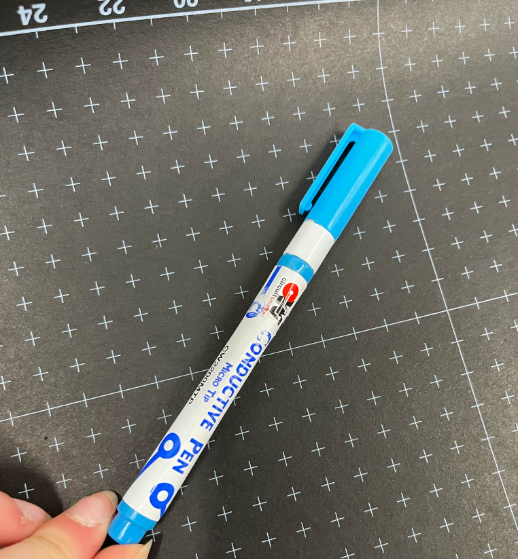
\includegraphics[width=\linewidth]{screenshot002}
		\caption{Paper conductor i retolador de tinta basada en una suspensió de plata.}
		\label{fig1.1a}
	\end{subfigure}
	\hfill
	\begin{subfigure}{0.45\textwidth}
		\centering
		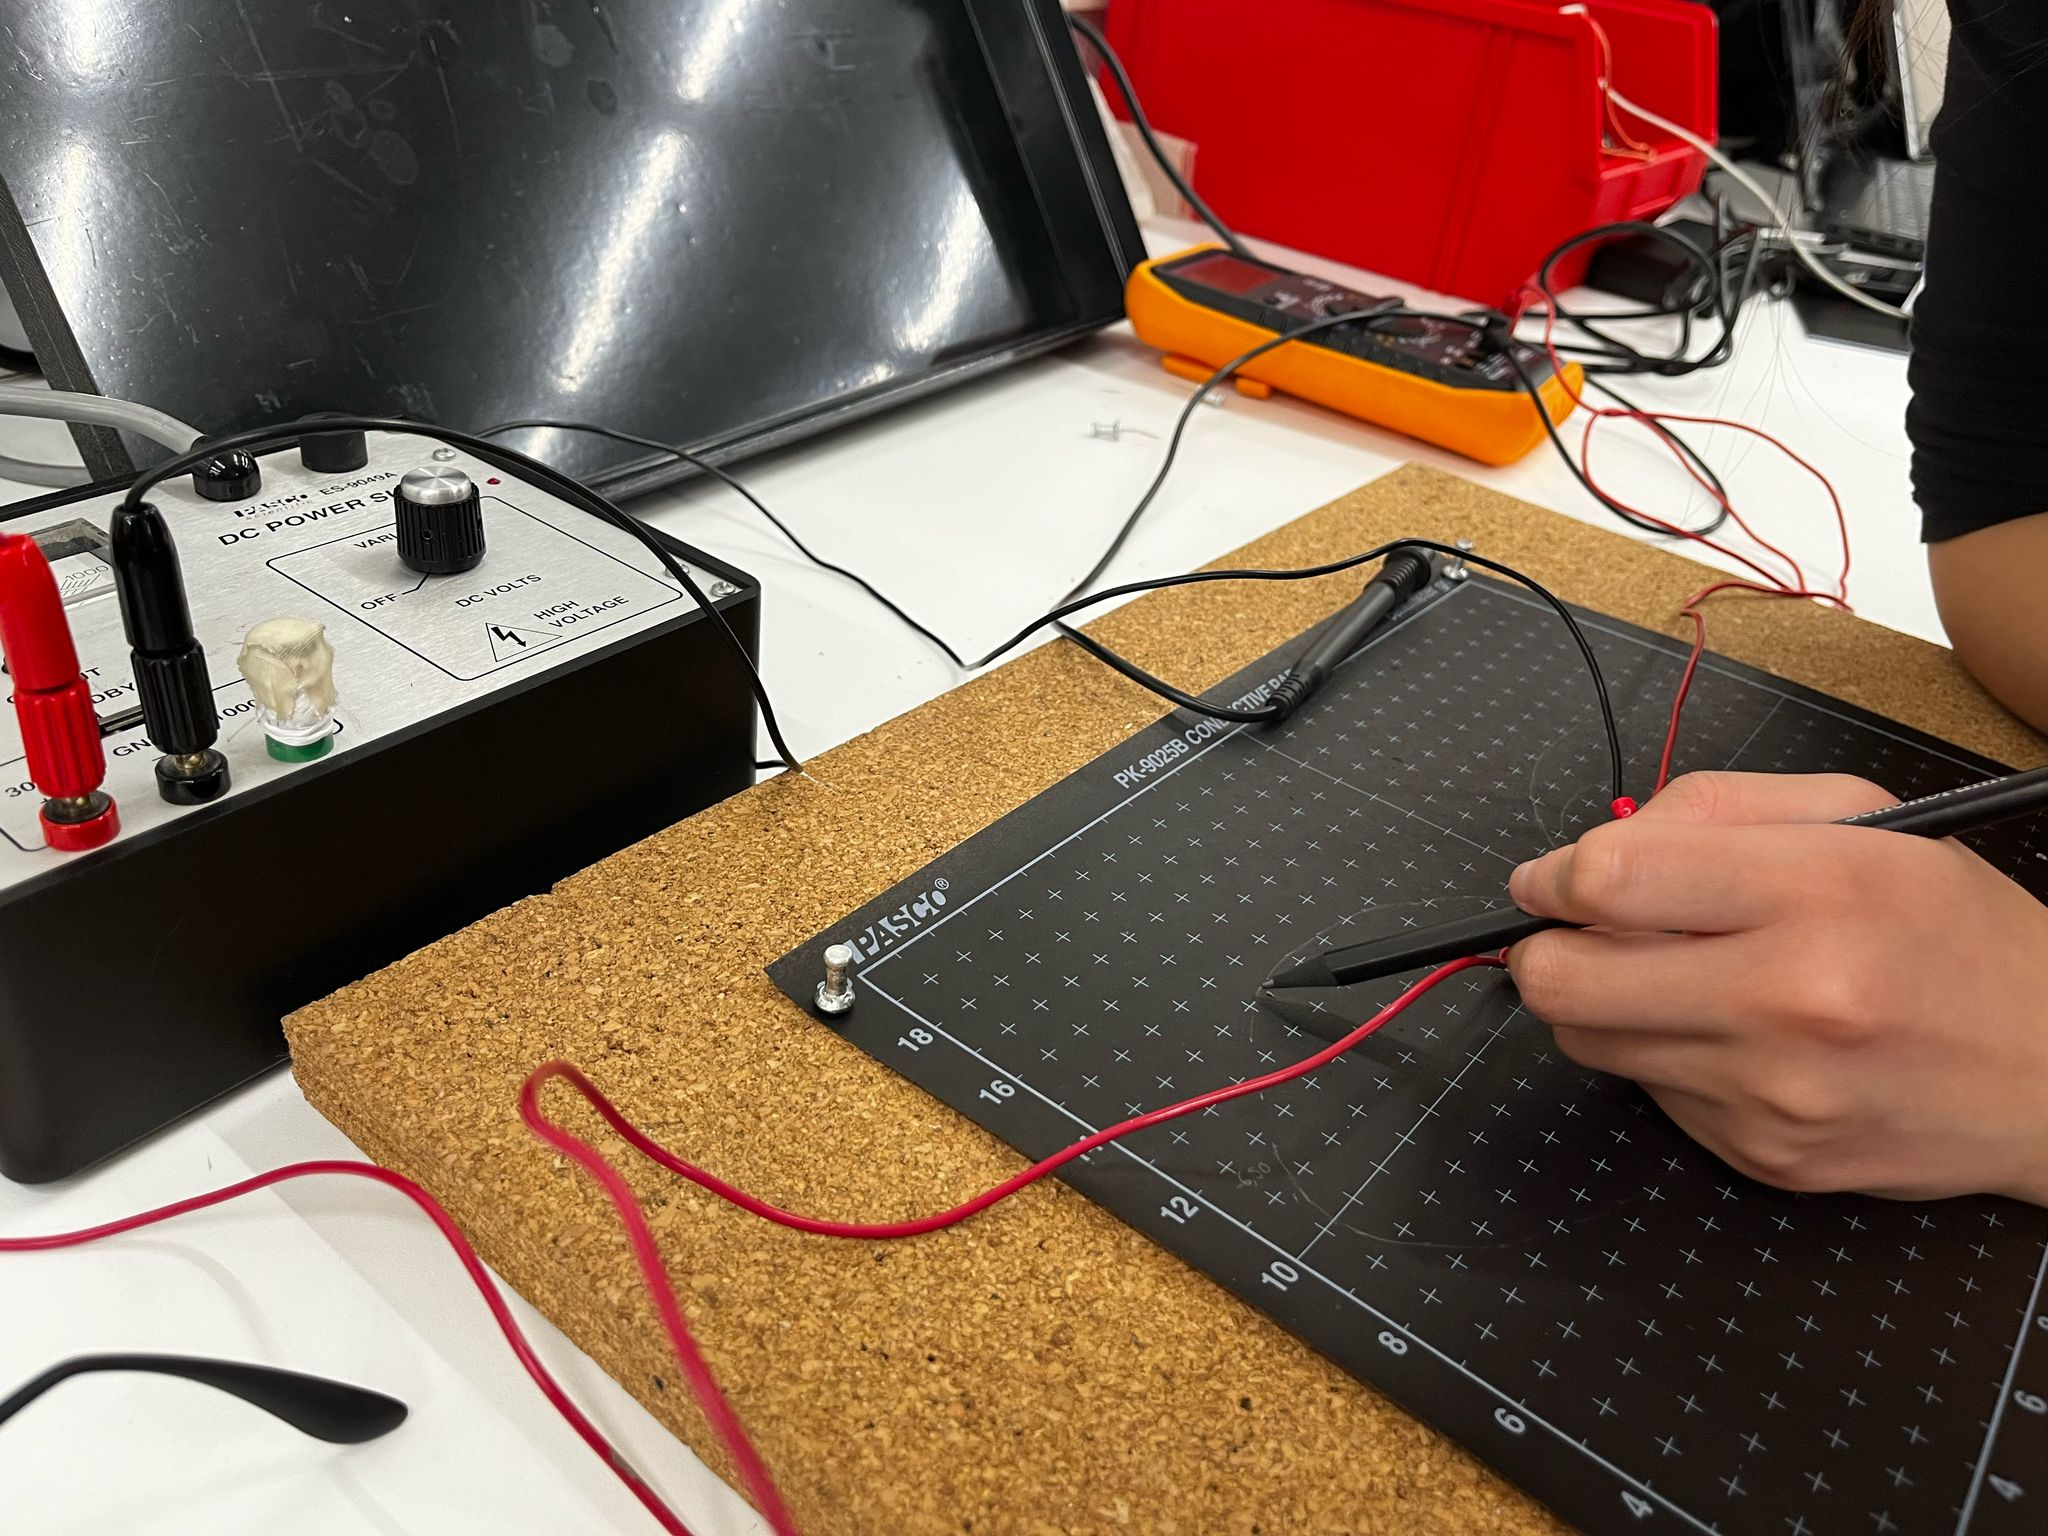
\includegraphics[width=\linewidth]{screenshot003}
		\caption{Muntatge experimental per a la representació de les corbes equipotencials pels dos fils infinits. D'esquerra a dreta: Font de corrent DC connectada als dos elèctrodes (dos punts pel cas representat) mitjançant dos cables; suro amb el paper conductor en el que prèviament s'han dibuixat els dos elèctrodes, enganxat amb xinxetes; multímetre usat per mesurar les diferències de potencial.}
		\label{fig1.1b}
	\end{subfigure}
	\caption{Paper conductor i muntatge experimental per a la representació de les corbes equipotencials.}
	\label{fig1.1}
\end{figure}

Hem treballat amb les següents tres distribucions: dues línies verticals (que són la projecció d'un condensador de plaques planoparal·leles), dos punts (projecció de dos fils infinits) i dues línies secants amb un punt entre elles (projecció de dos plans infinits formant angle d'aproximadament 60 º amb un fil infinit entre els dos).

Amb el pretext de generar el camp sobre les distribucions dibuixades, s'ha fixat el paper conductor (en el qual hem fet els dibuixos) sobre un suro usant xinxetes i hem connectat els elèctrodes (per a cada distribució per separat) a una font de corrent continu (DC) usant un parell de cables i més xinxetes. Per mesurar la diferència de potencial hem usat un multímetre, deixant un cable fixat a un dels dos elèctrodes (establint així una referència de potencial) i l'altre lliure per tal de fer mesures de $\Delta V$ a qualsevol altre punt del paper (veure figura \ref{fig1.1b}). Prèviament, però, ens hem assegurat què la diferència de potencial entre dos punts en els conductors (els elèctrodes dibuixats) no fos major de l'1\%\footnote{Recordem que, per ser aquests materials conductors, hem de tenir un potencial constant en tot el seu volum i, en particular, sobre la seva superfície.}.

Per dibuixar les corbes equipotencials usem el cable lliure del multímetre per buscar aquestes corbes sobre el paper. Marquem tots els punts que estan a un mateix potencial amb un llapis i, tot seguit, unim aquests punts amb una línia. Repetint això un seguit de cops podem construir vàries corbes equipotencials. Per tal d'assegurar-nos que es tanquen, és millor que comencem a buscar les corbes des de l'exterior dels nostres elèctrodes. Si comencem per l'interior, com que tindrem una densitat de corbes molt major, serà més fàcil que la línia escollida no s'acabi tancant. Veurem que ens interessa trobar corbes que tanquin els nostre elèctrodes per tal de poder aplicar el teorema de Gauss (en especial pel cas del condensador de plaques planoparal·leles).

Finalment, per representar el camp elèctric $\vec{E}$, hem dibuixat línies que sortien dels elèctrodes i tallaven les corbes equipotencials perpendicularment (en ambdós casos). 

\subsection{Càlcul de la capacitat del condensador}
Si aproximem la integral donada per l'equació \eqref{eq1.13} per un sumatori i calculem el camp $E_i$ segons
\begin{equation}
	E_i \approx \frac{\Delta V_i}{\Delta r_i} \label{eq1.14},
\end{equation}
on $\Delta r_i$ és la distància radial, $\Delta V_i$ és la diferència de potencial de l'element $\Delta l_i$, i el subíndex $i$ fa referència a la \textit{i-èssima} mesura. De tot això tenim:
\begin{equation}
	\frac{Q}{Z} \approx \varepsilon \sum_i \frac{\Delta V_i \Delta l_i}{\Delta r_i}.
\end{equation}
Usant que la capacitat d'un condensador de plaques planoparal·leles es correspon amb 
\begin{equation}
	C = \frac{Q}{\Delta V},
\end{equation}
la capacitat per unitat de longitud sota les aproximacions usades és:
\begin{equation}
	\frac{C}{Z} = \frac{Q/Z}{\Delta V} = \frac{\varepsilon}{\Delta V} \sum_i \frac{\Delta V_i \Delta l_i}{\Delta r_i} \label{eq1.17},
\end{equation}
on $\Delta V$ és la diferència de potencial a la qual hem sotmès les dues plaques del condensador.

\subsection{Distribució extra. Motivació}
Més enllà de les distribucions del condensador de plaques planoparal·leles i els dos fils infinits, treballem amb una tercera distribució: dos plans infinits secants (formant un angle de 60º) entre els quals tenim un fil infinit.

La raó per la qual hem decidit estudiar aquesta configuració és que ens servirà per comprovar si el mètode de les imatges és vàlid en aquest tipus de sistemes per tal de trobar la funció $\phi(\vec{r})$. El potencial generat per aquesta distribució es pot entendre com la superposició dels potencials creats per un conjunt de càrregues individuals distribuïdes adequadament (satisfent les mateixes condicions de contorn). En virtut del teorema d'unicitat, la solució de l'equació de Laplace de les dues distribucions és igual (llevat d'una constant), de forma que podem usar la darrera (més simple) per trobar el potencial de la primera (més complexa). 

A més a més, es pot demostrar fàcilment que en funció de l'angle d'intersecció entre els plans, la quantitat de càrregues imatge necessàries per reproduir el potencial del sistema variarà, satisfent que:
\begin{equation}
	N_q = \frac{360\text{º}}{\theta}-1 \label{eqimatges},
\end{equation}
on $N_q$ és el nombre de càrregues imatge i $\theta$ l'angle format pels dos plans. Fixem-nos en què $\theta = 180\text{º} \Rightarrow N_q = 1$, $\theta=90\text{º}\Rightarrow N_q =3$,$\dots$\footnote{Aquests són els resultats que vam veure en el problema 2.31 de la col·lecció de problemes de l'assignatura d'\textit{Electromagnetisme} (veure \cite{ref1}).} 
\subsection{Simulacions}
Els codis de les simulacions es poden trobar a l'annex \ref{an:a4}.

Per tal de simular el condensador planoparal·lel, considerem la distribució representada com la suma de doscentes càrregues puntuals (de valor $-q$ pel fil de l'esquerra i $q$ pel de la dreta) distribuïdes uniformement en les plaques, de manera que una es troba a $x = d/2$, i l'altra a $x = - d/2$. Pel que fa a l'eix de les ordenades, les càrregues estan situades des de $y = -H/2$ fins a $y = H/2$, on $H$ és l'alçada de la placa. Així, per a cada una de les càrregues, calculem la seva contribució al potencial i al camp elèctric en tots els punts de la malla $(X, Y)$ usant el principi de superposició.

Per la simulació dels dos fils infinits, considerem la seva projecció en el pla X$-$Y com dues càrregues puntuals separades una distància $d+2r$, essent aquest valor la separació entre els centres dels discos dibuixats experimentalment (de radi $r$).

Definim les funcions que descriuen el potencial i el camp elèctric corresponents a les expressions analítiques d'aquests magnituds per a una càrrega puntual. Així podem calcular la contribució de cada una en tots els punts de la malla aplicant el principi de superposició. D'aquesta manera obtenim el camp elèctric i el potencial total en cada punt de l’espai.

Per simular la tercera distribució de càrrega posem l'origen de coordenades en el punt on s'intersequen els plans i definim $d$ com la distancia en l'eix $x$ des de l'origen al fil infinit. A partir d'aquí, efectuem dues simulacions diferents:
\begin{itemize}
	\item En virtut del mètode de les imatges, podem substituir la nostra distribució per un conjunt de càrregues que satisfacin les condicions de contorn (potencial constant i igual a zero sobre els plans conductors); així doncs, simulem les corbes equipotencials i les línies de camp generades per cinc (veure equació \eqref{eqimatges}) càrregues imatge (i la real) a una distància $d$ de l'origen i separades entre elles 60º. Això és, però, assumint que els nostres plans són infinits.
	\item Per altra banda, simulem la nostra distribució per integració directa del potencial. Els detalls es poden trobar a l'annex \ref{an:a6}.
\end{itemize}

\section{Resultats i discussió}
Els resultats experimentals es poden trobar a l'annex \ref{an:a2}.

\subsection{Condensador de plaques planoparal·leles}
La primera configuració estudiada es correspon amb un condensador planoparal·lel, format per dos plans infinits (en l'eix Z, perpendicular al pla de la imatge) carregats i separats per una distància $d$. La seva projecció en el pla X$-$Y  resulta en dos fils infinits separats també per una distància $d$.

Les corbes equipotencials trobades experimentalment són les que es poden observar a la figura \ref{fig:1.2a}. Observem que dins la regió entre plaques, les línies equipotencials es mantenen gairebé paral·leles, indicant un camp elèctric gairebé uniforme i dirigit perpendicularment cap a les plaques. 

A les vores de les plaques, es manifesta l’efecte punta (degut a l'acumulació de càrregues a la superfície), on el camp deixa de ser uniforme i es distribueix de manera més complexa, amb línies equipotencials corbades cap a l’exterior. Aquest efecte és més acusat en condensadors de mida finita, ja que en el cas ideal de plaques infinites, el camp fora de la regió entre elles seria nul. Els resultats són, aproximadament els mateixos predits per la simulació de la figura \ref{fig:1.2b}.

Com ja hem comentat abans, podem utilitzar la llei de Gauss per tal de calcular la capacitat per unitat de longitud que tindria el condensador infinitament llarg en la direcció $Z$. Per fer-ho emprem l'expressió \eqref{eq1.17}, prèviament deduïda, i els resultats experimentals obtinguts en el transcurs de la pràctica\footnote{Aquests es poden trobar a la taula de l'annex \ref{an:a2}.}:
\begin{equation}
	\frac{C}{Z} = \frac{Q/Z}{\Delta V} = \frac{\varepsilon}{\Delta V} \sum_i \frac{\Delta V_i \Delta l_i}{\Delta r_i} = (2,06 \pm 0,21)\varepsilon \text{ F/m}.
\end{equation}
Podem comparar aquest resultat amb el que s'obtindria si tinguéssim un condensador ideal de plaques planoparal·leles si usem que\footnote{Les mesures per $H$ i $d$ s'han efectuat digitalment amb \textit{ImageJ}.}:
\begin{equation*}
	H = (7,961\pm0,001) \text{ cm}, \hspace{0.25cm} d = (5,598\pm0,001) \text{ cm}.
\end{equation*}
De manera que:
\begin{equation}
	\frac{C}{Z} = \frac{A\varepsilon/d}{Z} = \frac{H}{d}\varepsilon = (1,4221 \pm 0,0003)\varepsilon \text{ F/m},
\end{equation}
on $A$ es l'àrea de la placa i $H$ l'altura d'aquesta. 
Veiem que el nostre condensador es desvia notablement del cas ideal. És més, segons els nostres càlculs, el condensador real té una capacitat per unitat de longitud superior, cosa que, a priori, no pot ser. 

Hi ha principalment dos motius pels quals no hem obtingut la càrrega per unitat de longitud real: Primer, experimentalment hauríem d'haver fet més punts per tal tenir unes línies de camp més precises i així poder fer una millor aproximació a la integral donada per \eqref{eq1.17}; segon, i més important, perquè aquesta aproximació sigui lo més bona possible, cal que la suposició donada per l'equació \eqref{eq1.14} sigui també molt bona, i per tal que això sigui així, cal que les línies equipotencials mesurades experimentalment siguin molt properes, ja que, per poder assegurar que
\begin{equation}
	E = \frac{\partial V_i}{\partial r_i} \approx \frac{\Delta V_i}{\Delta r_i},
\end{equation}
és necessari que el $\Delta r_i$ entre les corbes equipotencials sigui suficientment petit com per que $\Delta r_i \rightarrow \partial r_i$ i que, a més a més, estigui en al direcció perpendicular a les corbes equipotencials, per tal de poder dir que la suposició donada a \eqref{eq1.14} és vàlida. En el nostre cas, òbviament això no és estrictament correcte, ja que la separació entre les línies equipotencials no és negligible i el $\Delta r_i$ no necessàriament és perpendicular a aquestes. 

\begin{figure}
	\centering
	\begin{subfigure}{0.45\linewidth}
		\centering
		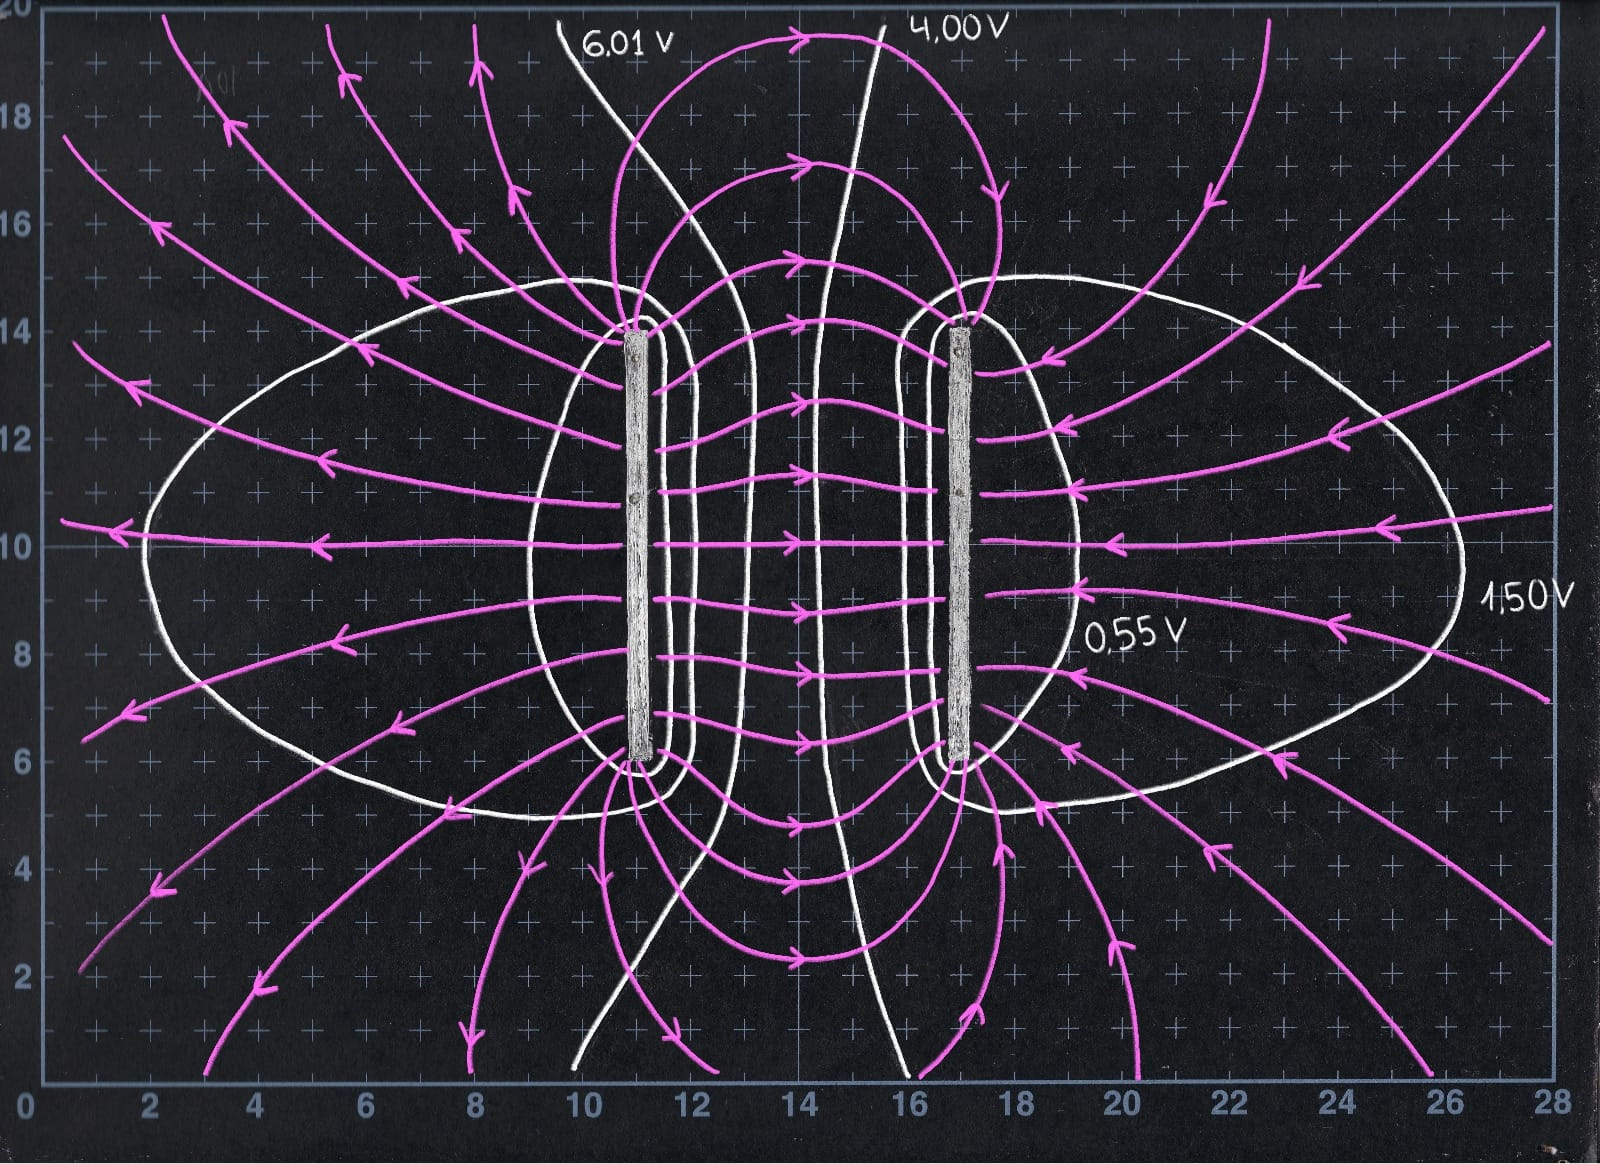
\includegraphics[height=5.5cm]{dibplaques} % Augmenta la mida
		\caption{Corbes equipotencials (en blanc) i línies de camp $\vec{E}$ (en lila) pel cas del condensador planoparal·lel trobades experimentalment.}
		\label{fig:1.2a}
	\end{subfigure}
	\hfill
	\begin{subfigure}{0.53\linewidth}
		\centering
		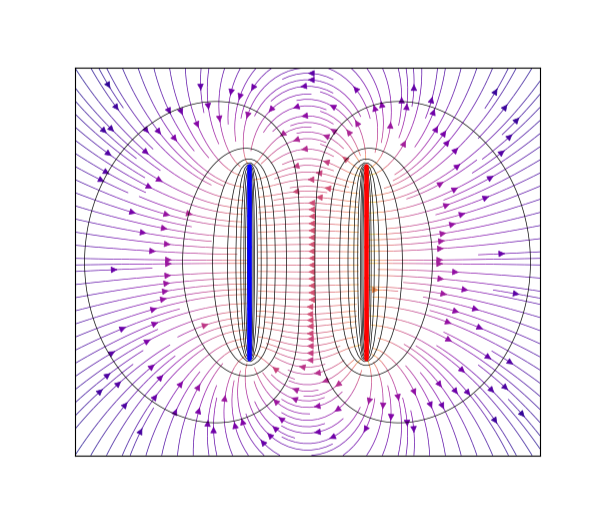
\includegraphics[height=6.5cm]{figplaques1} % Mateixa alçada
		\caption{Simulació del camp elèctric i del potencial pel condensador planoparal·lel.}
		\label{fig:1.2b}
	\end{subfigure}
	\caption{Representació i simulació de les corbes equipotencials i línies de camp per la distribució associada al condensador planoparal·lel.}
	\label{fig:1.2}
\end{figure}


\subsection{Fils infinits}
La segona configuració estudiada és la projecció en el pla X$-$Y (pla de la imatge) de dos fils infinits separats per una distància constant. 

Les corbes equipotencials trobades experimentalment són les que es poden observar a la figura \ref{fig:1.3a}. Observem com aquestes formen el·lipses on els fils estan cada cop més descentrats conforme agafem corbes més externes. 
\begin{figure}[h]
	\centering
	\begin{subfigure}{0.45\linewidth}
		\centering
		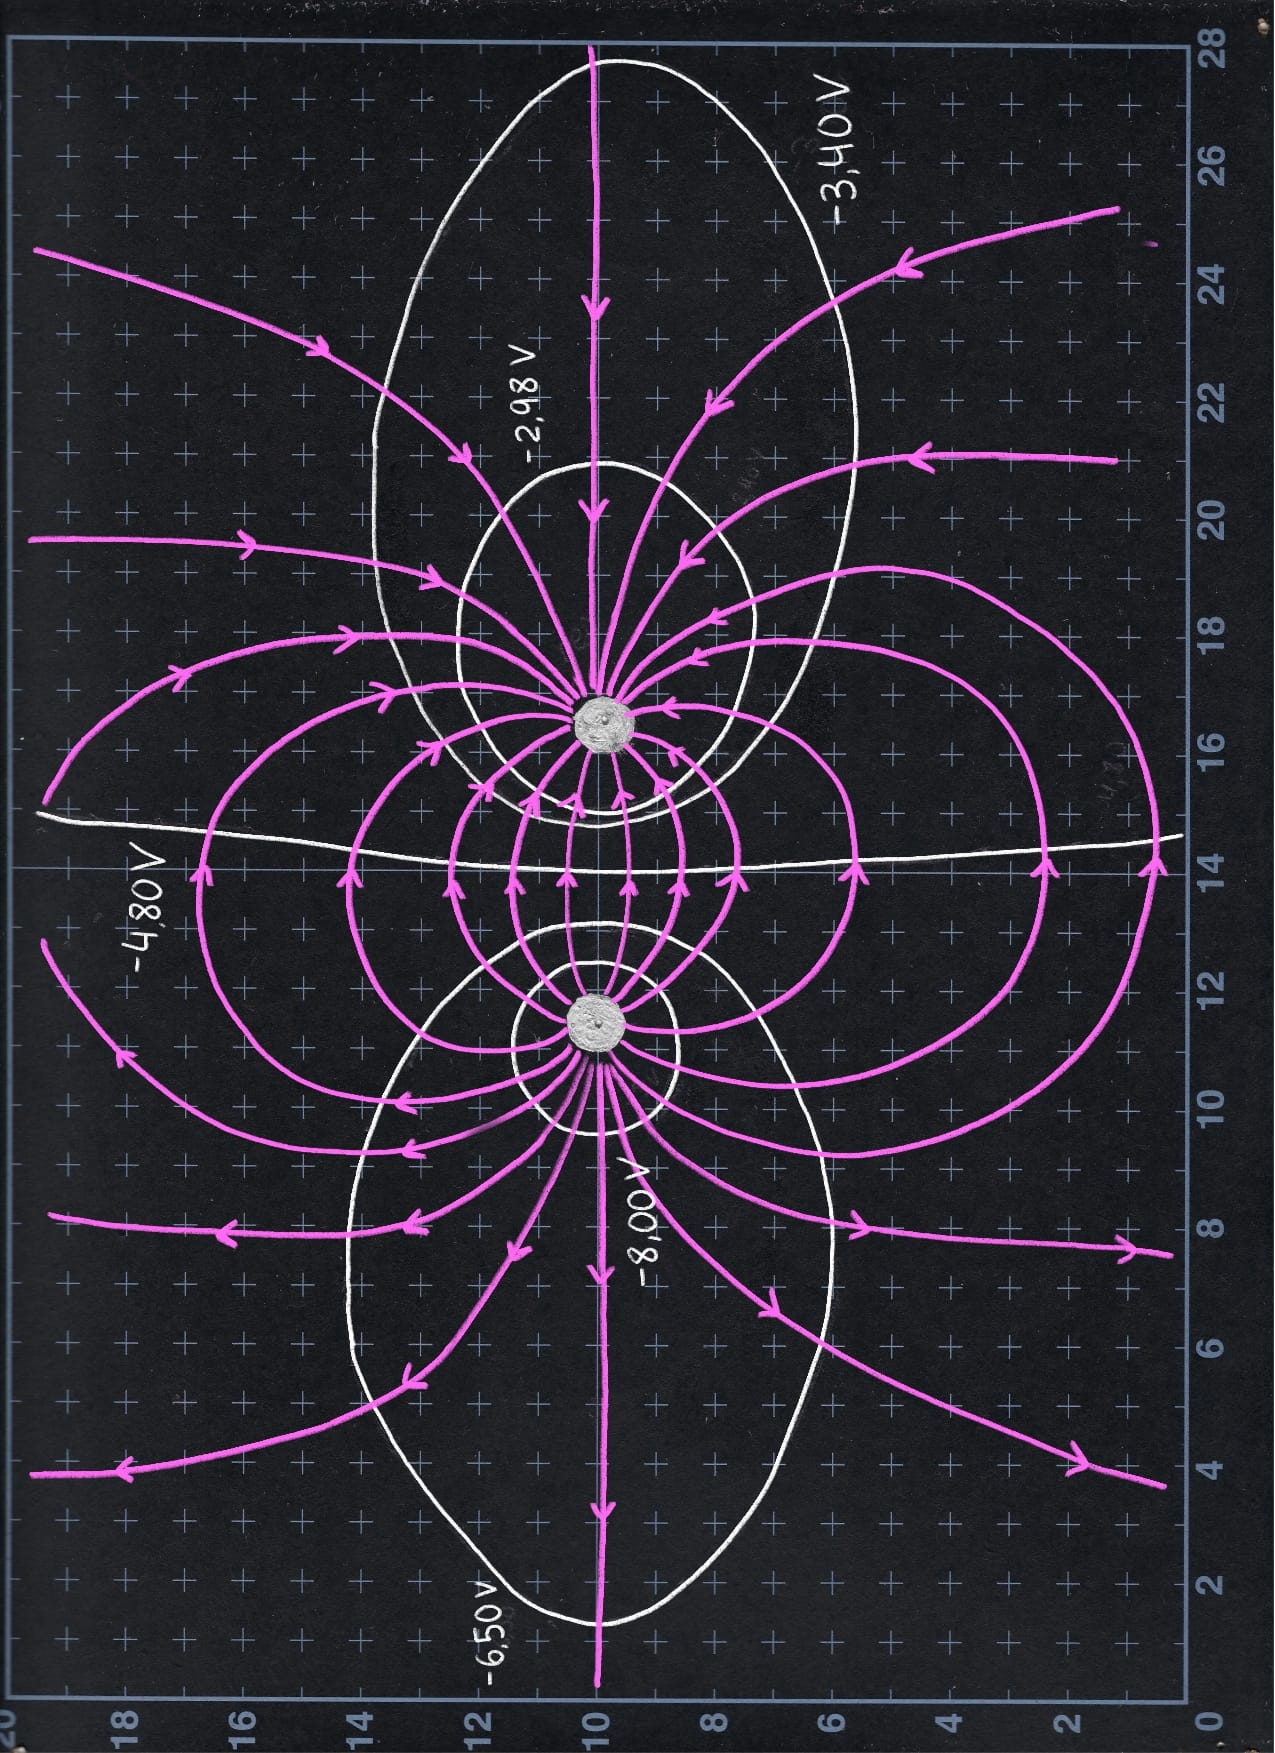
\includegraphics[width=\linewidth]{screenshot004}
		\caption{Corbes equipotencials (en blanc) i línies de camp $\vec{E}$ (en lila) pel cas dels dos fils infinits trobades experimentalment.}
		\label{fig:1.3a}
	\end{subfigure}
	\hfill
	\begin{subfigure}{0.5\linewidth}
		\centering
		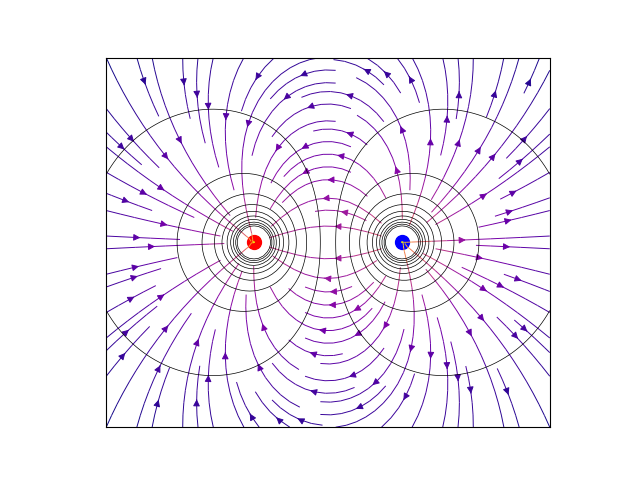
\includegraphics[width=\linewidth]{figfils}
		\caption{Simulació del camp elèctric i del potencial pels dos fils infinits.}
		\label{fig:1.3b}
	\end{subfigure}
	\caption{Representació i simulació de les corbes equipotencials i línies de camp per la distribució de dos fils infinits.}
	\label{fig:1.3}
\end{figure}

Els resultats teòrics indiquen que, en un sistema de dos fils infinits, les corbes equipotencials venen donades per la següent equació:
\begin{equation}
	y^2+\left( x+a\frac{1+k^2}{1-k^2}\right)^2 = a^2\left( \frac{2k}{1-k^2}\right)^2  \label{eqsuppon},
\end{equation}
que és l'equació d'una circumferència. Per tant, les corbes equipotencials teòriques haurien de ser circumferències de radi $R = a\frac{2k}{1-k^2}$ amb el centre lleugerament desplaçat en l'eix de les $x$ per un factor $a\frac{1+k^2}{1-k^2}$. Notem que tant $a$ com $k$ són dues constants\footnote{Els valors de les constants i la demostració d'aquest resultat es pot trobar a l'annex \ref{an:a1}.}. Es pot veure que es compleix exactament el que s'ha descrit atenint-nos als resultats obtinguts a la simulació de la figura \ref{fig:1.3b}.

El fet que els nostres resultats es desviïn del predit per la teoria es deu als diferents errors experimentals comesos durant l'evolució de la pràctica. Els principals factors que poden alterar els resultats de l'experiment són: s'assumeix que el paper conductor té una conductivitat $\sigma$ homogènia, però això no necessàriament ha de ser així (pot ser que presenti inhomogeneïtats), els punts que representen la projecció dels dos fils infinits en el pla no són perfectament rodons, ja que han sigut dibuixats a mà (amb les imprecisions que això comporta). Pel que fa a les corbes equipotencials i les línies de camp, aquestes es poden veure afectades per l'efecte punta a les vores dels materials carregats, on s'acumula més densitat de càrrega. 


\subsection{Fil infinit i dos plans}

La tercera configuració estudiada i proposada per nosaltres és la projecció en el pla X$-$Y de dos plans infinits (en l'eix $Z$) formant un angle de $60^o$ amb més un fil infinit (en l'eix $Z$) situat dins de la regió entre els plans.

Les corbes equipotencials trobades experimentalment són les que es poden observar a la figura \ref{fig:1.4a}.

\begin{figure}[h]
	\centering
	\begin{subfigure}{0.49\linewidth}
		\centering
		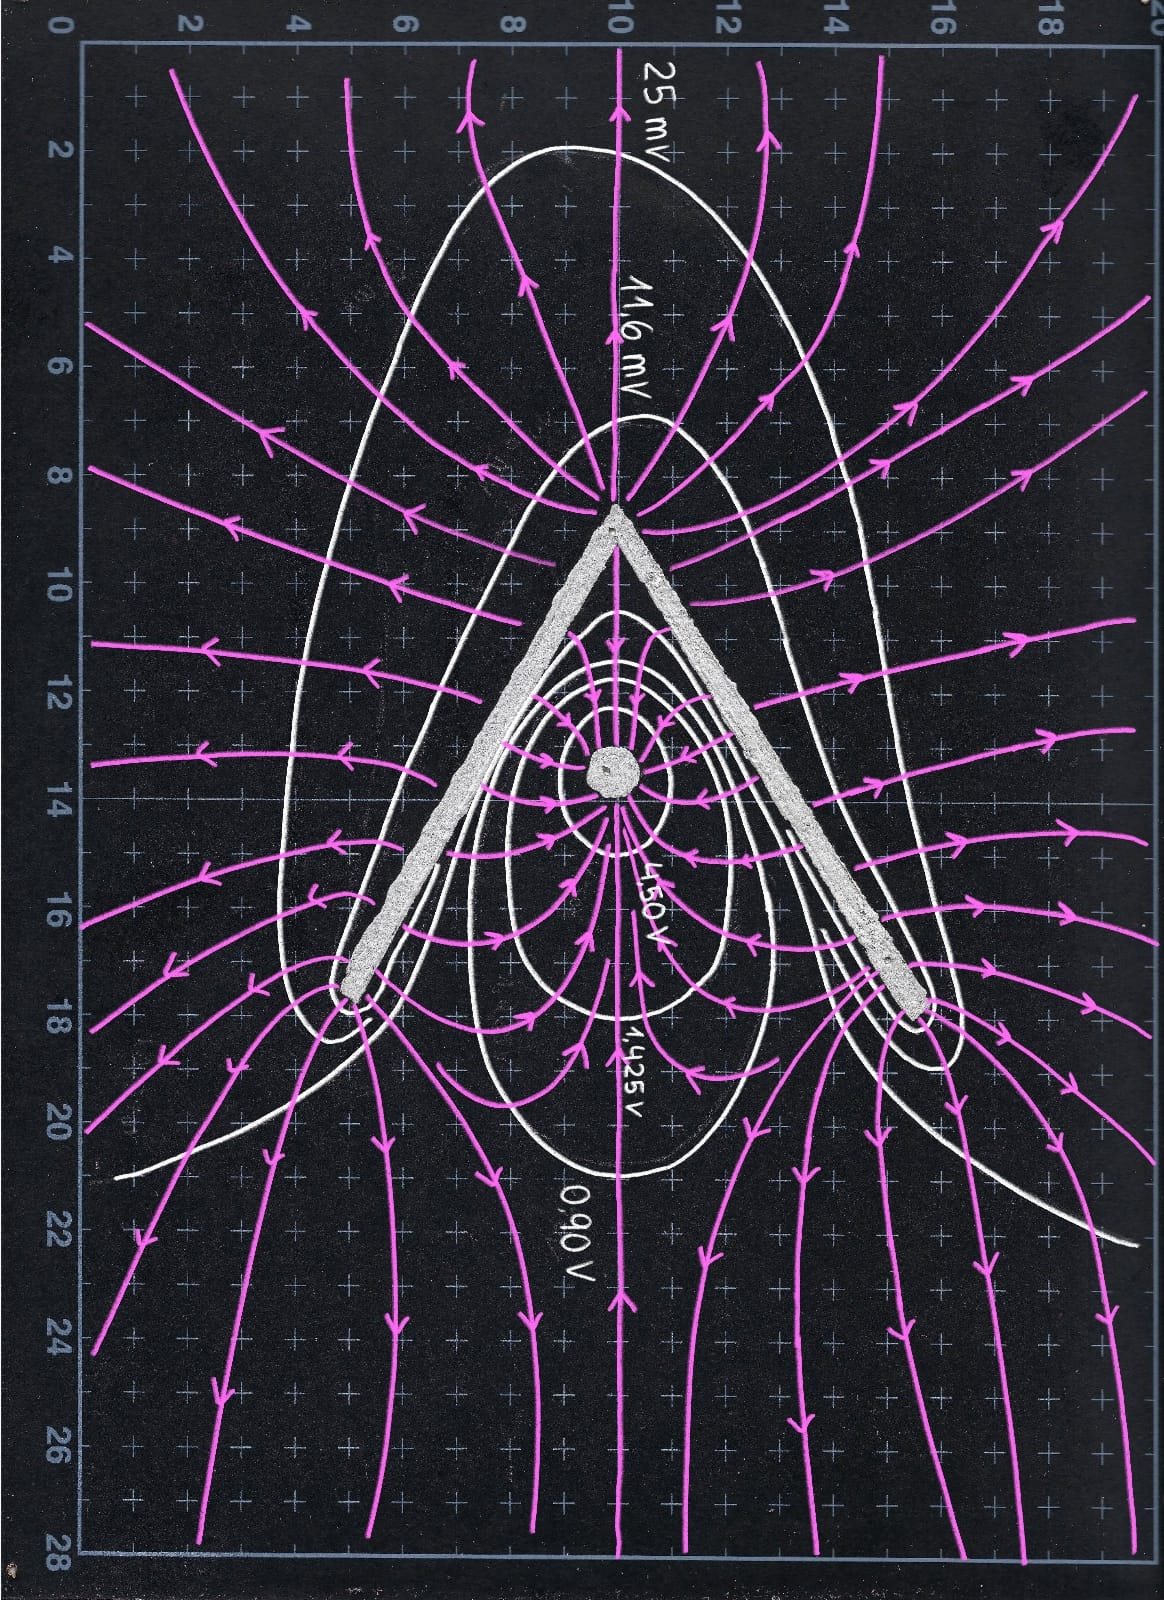
\includegraphics[width=\linewidth]{confinventJS}
		\caption{Corbes equipotencials (en blanc) i línies de camp $\vec{E}$ (en lila) pel cas dels dos plans infinits i un fil infinit trobades experimentalment.}
		\label{fig:1.4a}
	\end{subfigure}
	\hfill
	\begin{subfigure}{0.49\linewidth}
		\centering
		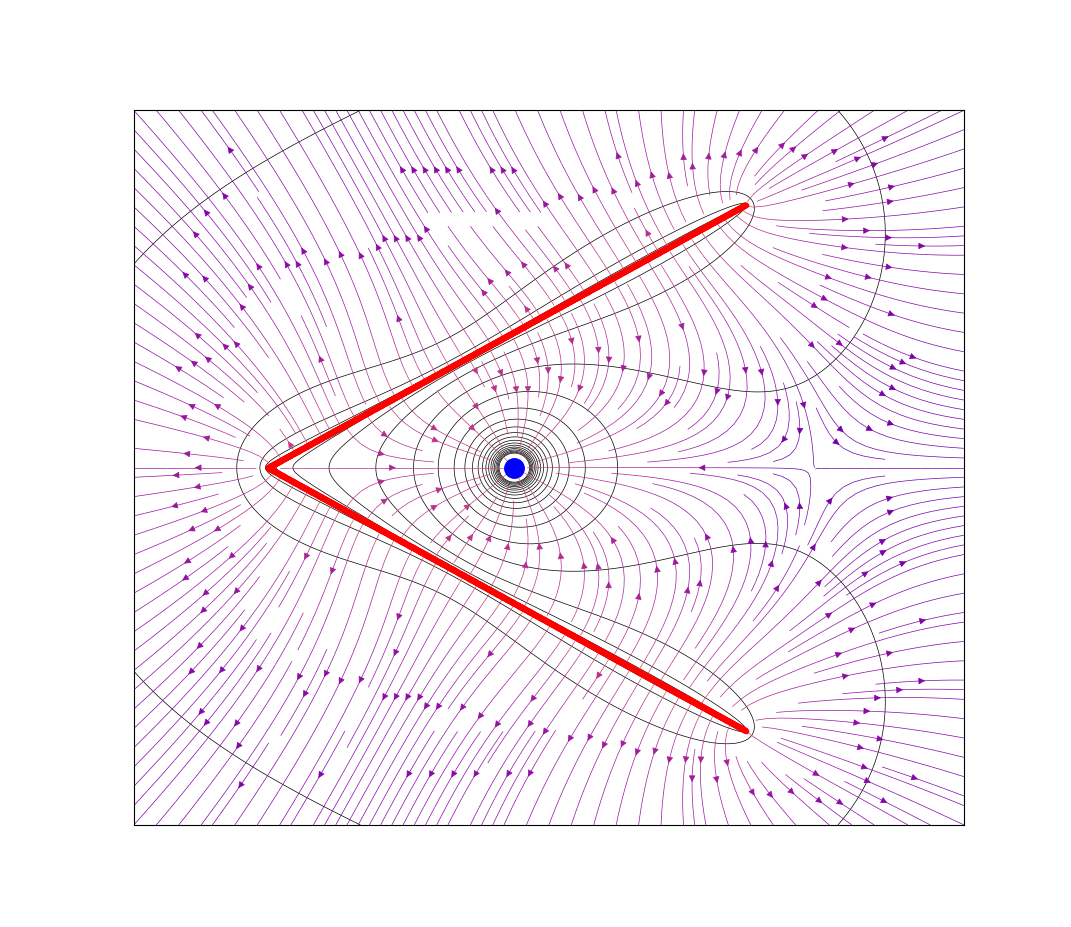
\includegraphics[width=\linewidth]{figplacarara}
		\caption{Simulació del camp elèctric i del potencial pels dos plans i el fil infinit.}
		\label{fig:1.4b}
	\end{subfigure}
	\caption{Representació i simulació de les corbes equipotencials i línies de camp per la distribució de dos plans infinits amb un fil infinit enmig.}
	\label{fig:1.4}
\end{figure}

Notem que aquesta configuració de càrrega és molt més complexa que les anteriors, ja que una de les distribucions, pel fet de ser triangular, l'efecte punta es fa molt notable als extrems. De fet, veiem que en aquests punts el camp divergeix molt més que en altres regions.

\begin{figure}[h]
	\centering
	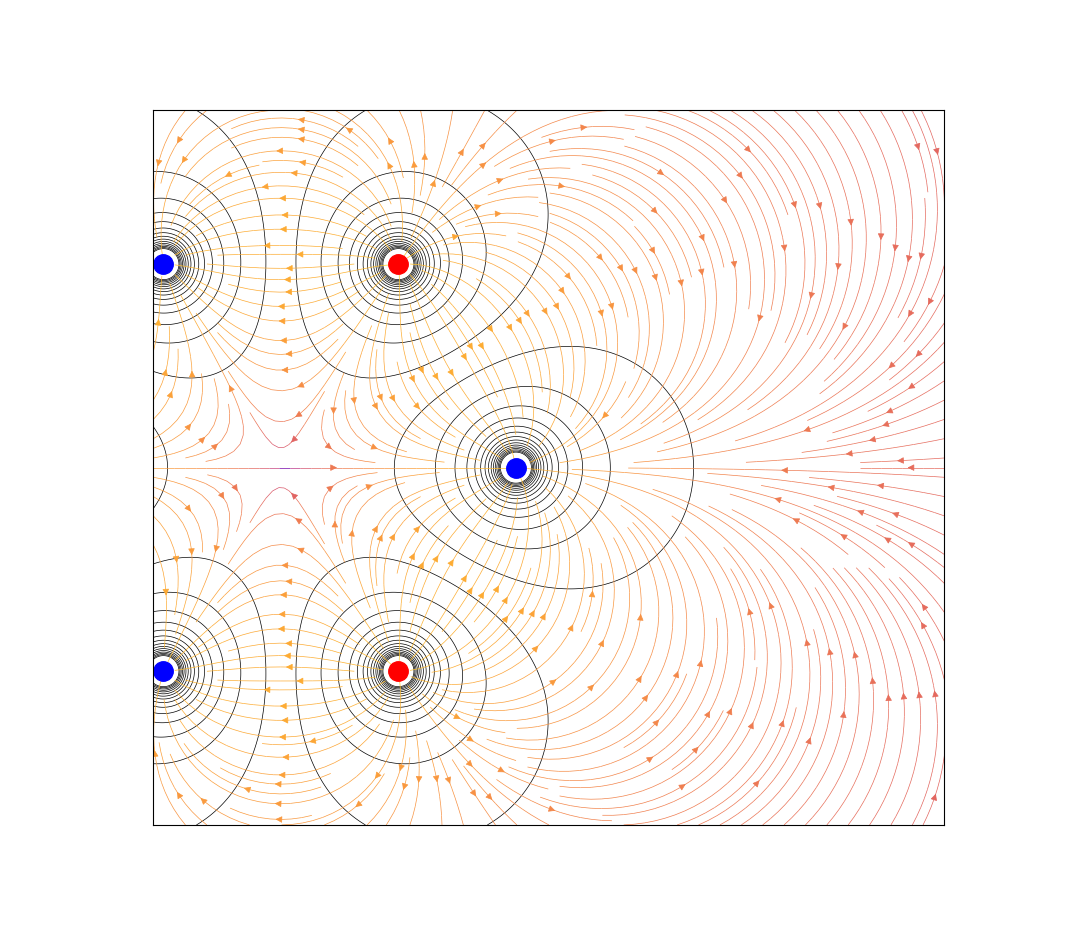
\includegraphics[width=0.45\linewidth]{figV2imagenes}
	\caption{Simulació de les corbes equipotencials i de les línies de camp elèctric associades a la distribució de càrregues imatge solució.}
	\label{fig:1.5}
\end{figure}

Hem fet la simulació pel mètode de les imatges que presentem a la figura \ref{fig:1.5}. Aquesta presenta un comportament molt similar a l'obtingut experimentalment. Pel que fa a la regió entre la càrrega i les plaques, els resultats són pràcticament idèntics, però conforme ens allunyem de la càrrega, el comportament comença a diferir. Podem trobar un clar exemple fixant-nos en punts situats sobre l'eix de les abscisses amb un valor de $x$ gran. En aquesta regió, tant en la representació experimental com en l'analítica, el camp apunta cap a fora de la distribució, metre que en la simulació pel mètode de les imatges és al revés.

Les diferències esmentades posen de manifest que la solució trobada a partir del mètode de les imatges no pot ser comparada a determinades regions de l'espai, principalment perquè aquesta solució considera les plaques infinites (i clarament les nostres no ho són). Per tant, la comparació amb els  resultats experimentals només té sentit si ens trobem dins del món real però mantenint-nos a les proximitats del fil.


\section{Conclusions}
Aquesta pràctica s'ha basat en l'ús d'un multímetre per tal de mesurar el potencial elèctric a diferents distàncies de les distribucions de càrrega dibuixades. Això ens ha permès, per una banda, traçar línies equipotencials i, per altra, obtenir un valor de la capacitat per unitat de longitud d'un condensador.

Pel que fa a les línies equipotencials, aquestes ens han servit de guia per dibuixar, posteriorment, les respectives línies de camp elèctric, ja que, com sabem de teoria, aquestes són perpendiculars a les equipotencials. A més a més, per a les tres geometries considerades, hem generat les corresponents simulacions basades en mètodes numèrics amb més facilitat. Així podem comparar els resultats experimentals amb els teòrics amb més facilitat.

Addicionalment, per a la tercera distribució (dos plans secants i un fil infinit), com que coneixíem la solució que ens dona el mètode de les imatges (motiu pel qual l'hem escollit), hem pogut contrastar les línies equipotencials i de camp trobades experimentalment amb les del mètode mencionat, verificant així la validesa d'aquesta solució.

Tal i com s'ha anat mencionant, tant les línies equipotencials com les de camp basades en les mesures del multímetre (resultats experimentals) segueixen la mateixa tendència que les simulacions. Tot i no coincidir-hi exactament a causa de l'efecte punta i els possibles errors aleatoris associats (inhomogeneïtats del paper, haver dibuixat formes irregulars, imprecisions causades pel gruix de la punta del llapis,...), la geometria i el sentit de les línies de camp són coherents.

Per altra banda, hem calculat la capacitat per unitat de longitud d'un condensador de plaques planoparal·leles a partir del teorema de Gauss. Com s'ha explicat, el càlcul experimental s'ha realitzat amb un sumatori com a aproximació de la integral de l'equació \ref{eq1.13}. Atès que el resultat obtingut és coherent amb el valor teòric esperat, podem considerar vàlida l'aproximació emprada.

Així, a partir de tres distribucions de conductors diferents amb suficient simetria com per reduir el problema a dues dimensions, hem comprovat l'existència de la dualitat entre la densitat de corrent $\vec{J}$ i el vector desplaçament $\vec{D}$.

\chapter{Força entre corrents}
\begin{chapterabstract}
	En aquesta pràctica mesurem la força entre dos fils pels quals hi circula un corrent elèctric, comprovant que la llei de Biot i Savart se satisfà, via diferents metodologies. Amb aquests resultats fem una estimació de la permeabilitat magnètica $\mu_0$, tot comparant-la amb el valor teòric. A més a més, utilitzant el mateix sistema, mesurem la component horitzontal del camp magnètic terrestre al laboratori.
\end{chapterabstract}
\section{Introducció i fonament teòric}
Per quantificar la interacció magnètica entre dos circuits arbitraris tancats pels quals hi circula un corrent constant, és a dir, per mesurar la força que fa un circuit sobre l'altre podem usar que
\begin{equation}
	\vec{F}_1 = \frac{\mu_0}{4\pi}I_1I_2\oint \oint \frac{\mathrm{d}\vec{l}_1\cross[\mathrm{d}\vec{l}_2 \cross (\vec{r}_1-\vec{r}_2)]}{\abs{\vec{r}_1 - \vec{r}_2}^3}\label{eq:2.1},
\end{equation}
on $\mu_0$, $I_1$ i $I_2$ són les intensitats dels circuits 1 i 2, respectivament, d$\vec{l}_1$ i d$\vec{l}_2$ són els elements infinitesimals de línia i $\vec{r}_1$ i $\vec{r}_2$ són les respectives posicions d'aquests elements.

Per tal de simplificar la integral anterior definim el camp d'inducció magnètica (o densitat de flux magnètic) $\vec{B}(\vec{r})$ en un punt arbitrari $\vec{r}$ com
\begin{equation}
	\vec{B}(\vec{r}) = \frac{\mu_0}{4\pi} \int_V \vec{J}(\vec{r}_1)\cross\frac{\vec{r}-\vec{r}'}{\abs{\vec{r}-\vec{r}'}^3}\mathrm{d}^3r'.
\end{equation} 
Si usem això sobre l'equació \eqref{eq:2.1} podem escriure la força que rep el circuit amb intensitat I degut a la presència del camp d'inducció $\vec{B}$ creat per l'altre circuit segons
\begin{equation}
	\vec{F} = I \oint \mathrm{d}\vec{l}\cross\vec{B}(\vec{r}).
\end{equation}
Emprant una de les equacions pel camp $\vec{B}$
\begin{equation}
	\vec{\nabla}\cross \vec{B} = \mu_0 \vec{J},
\end{equation}
i aplicant el teorema de Stokes
\begin{equation}
	\oint_C \vec{A} \cdot \mathrm{d}\vec{r} = \int_S (\vec{\nabla}\cross \vec{A})\cdot \mathrm{d}\vec{S},
\end{equation}
podem deduir fàcilment el teorema d'Ampère, que ens diu que:
\begin{equation}
	\oint_C\vec{B}\cdot\mathrm{d}\vec{l} = \mu_0\int_S\vec{J}(\vec{r})\cdot\vec{n}\mathrm{d}S,
\end{equation}
d'on, mitjançant un càlcul ràpid podem trobar el camp d'inducció magnètica generat per un fil infinit amb intensitat $I$ a una distància $r$ del seu centre
\begin{equation}
	B = \frac{\mu_0 I}{2\pi r}.
\end{equation}
Així doncs, la força, en mòdul que patirà un altre fil (infinit) paral·lel, de longitud $L$ i que és perpendicular al camp $\vec{B}$ serà
\begin{equation}
	F = \frac{\mu_0 I^2L}{2\pi r}.
\end{equation} 
\section{Metodologia experimental}

\subsection{Equilibrat de la balança}
\subsection{Força vs. corrent}
\subsection{Força vs. separació}
\subsection{Mesura del camp magnètic terrestre}

\section{Resultats i discussió}

\subsection{Valor experimental de la permeabilitat magnètica}
\subsection{Camp magnètic terrestre}

\section{Conclusions}


\chapter{Circuit RLC en sèrie}

\begin{chapterabstract}
	En aquesta pràctica estudiem el comportament del circuit més elemental que presenta oscil·lacions: el circuit RLC (resistència + condensador + bobina) en serie. El nostre objectiu principal és visualitzar, mitjançant un oscil·loscopi, les diferents solucions de l'equació diferencial de segon ordre associada a aquest sistema de gran interès físic.
\end{chapterabstract}

\section{Introducció i fonament teòric}

\subsection{Explicació qualitativa}
ESQUEMA DEL CIRCUIT + LINK A ANIMACIÓ DE LA WIKIPEDIA

Per entendre per què aquest tipus de circuits presenten oscil·lacions considerem, inicialment, que no tenim cap resistència i que el condensador es troba totalment carregat. En connectar les plaques del condensador a la bobina, comença a circular una intensitat $I$ per aquesta. La variació de $I$ provoca, en virtut de la llei de Lenz
\begin{equation}
	\varepsilon = - \dv{}{t}\int_S \vec{B} \cdot \mathrm{d}\vec{s} \label{eq:3.1},
\end{equation}
una força electromotriu induïda als extrems de la bobina que s'oposa a l'augment de corrent. Com que la resistència $R$ és nul·la el potencial a la bobina serà igual i de signe contrari al potencial entre les plaques del condensador (si no fos així tindríem una intensitat infinita circulant per la bobina). 

Tanmateix, mentre el condensador es descarrega, la intensitat va augmentant, de forma que, quan el condensador està totalment descarregat (i, per tant, el potencial és zero entre les dues plaques), la intensitat és màxima. Com que és impossible que el corrent s'anul·li de sobte (ja que implicaria una $\varepsilon$ infinita), continua circulant intensitat en el mateix sentit i el condensador es carrega amb polaritat contrària a la de l'inici. 

Ara, el procés de càrrega del condensador fa que la intensitat disminueixi progressivament (el voltatge total del circuit ha de ser nul en tot moment); quan la intensitat arriba a zero la càrrega del condensador ha de ser necessàriament la mateixa que a l'inici, ja que, com que la resistència òhmica del circuit és nul·la, no hem tingut pèrdues energètiques associades a l'efecte Joule, però el potencial és de signe oposat. En tot aquest procés ha passat un \textit{semiperíode}. Seguidament torna a començar el procés de càrrega del condensador fins a tornar a arribar a la situació inicial; tot plegat explica per què el voltatge entre les plaques del condensador oscil·la indefinidament.

La capacitat $C$ del condensador és
\begin{equation}
	C = \frac{q}{V_C}, \label{eq:3.2}
\end{equation}
i l'autoinductància de la bobina és
\begin{equation}
	L = V_L \frac{\Delta t}{\Delta I}, \label{eq:3.3}
\end{equation}
on $q$ és la càrrega emmagatzemada al condensador, el quocient $\frac{\Delta t}{\Delta I}$ és la variació de temps per una certa variació de la intensitat i  $V_L$ i $V_C$ són els voltatges associats a la bobina i al condensador, respectivament. Aquestes dues magnituds, que depenen únicament de la geometria del sistema considerat, són de vital importància per descriure com seran aquestes oscil·lacions. Notem que: 
\begin{itemize}
	\item Com més petita sigui la capacitat $C$ del condensador, més ràpidament es descarregarà (té menys càrrega).
	\item Com més petita sigui l'autoinductància $L$ de la bobina, més variació en la intensitat és necessària per donar una mateixa força electromotriu $\varepsilon$, de manera que també més ràpidament es descarregarà el condensador.
\end{itemize}
Si tenim presents aquests dos efectes, fàcilment podem arribar a la conclusió que com menors siguin l'autoinductància i la capacitat del circuit, més alta serà la freqüència d'oscil·lació.

Totes aquestes consideracions són assumint que la resistència del circuit és negligible. En cas que no ho sigui (com en el cas que estudiem) el voltatge a la bobina i al condensador seran lleugerament diferents i, per cada oscil·lació, perdrem part de l'energia del sistema en forma de calor (per l'efecte Joule). Si la resistència es fa molt gran, deixaran d'haver-hi oscil·lacions.

\subsection{Equació general del circuit RLC}
Per circuits en sèrie els voltatges se sumen i les intensitats són iguals per a tots els elements del circuit, de forma que el voltatge total es correspondrà amb
\begin{equation}
	V = V_R + V_L + V_C = RI + L \dv{I}{t} + \frac{1}{C} \int I\mathrm{d}t, \label{eq:3.4}
\end{equation}
on hem emprat les expressions 
\begin{align}
	V_R & = RI, \\
	V_L & = L \dv{I}{t}, \\
	V_C & = \frac{1}{C} \int I \mathrm{d}t.
\end{align}
Si derivem respecte del temps l'expressió \eqref{eq:3.4} i reorganitzem obtenim:
\begin{equation}
	\dv[2]{I}{t} + \frac{R}{L} \dv{I}{t}+\frac{1}{LC} = \frac{1}{L}\dv{V}{t}.\label{eq:3.8}
\end{equation}
Podem trobar dues expressions alternatives a aquesta darrera equació. Si ens interessa tenir una equació en funció del potencial als extrems de la resistència només cal que multipliquem per $R$; si ens interessa expressar-ho tot en funció del potencial al condensador hem de tenir en compte que
\begin{equation}
	I = C \dv{V_C}{t},
\end{equation}
de manera que obtenim les següents dues expressions alternatives:
\begin{align}
	\dv[2]{V_R}{t} + \frac{R}{L}\dv{V_R}{t} + \frac{1}{LC}V_R = \frac{R}{L} \dv{V}{t}, \\
	\dv[2]{V_C}{t} + \frac{R}{L}\dv{V_C}{t} + \frac{1}{LC}V_C=\frac{1}{LC}V. \label{eq:3.11}
\end{align}

\subsection{Règim permanent}
En aquest règim assumim que subministrem un senyal sinusoidal al circuit, de manera que:
\begin{equation}
	V(t) = V_{max} \sin (\omega t). \label{eq:3.12}
\end{equation} 
La solució de l'equació \eqref{eq:3.8} és també una ona sinusoidal:
\begin{equation}
	I(t) = I_{max}\sin(\omega t + \phi).
\end{equation}
Si expressem això en notació complexa\footnote{Denotem la unitat imaginària amb $j$ per evitar confusions amb la intensitat.}
\begin{align}
	I(t) & = I_{max} \mathrm{e}^{j(\omega t + \phi)}, \\
	V(t) & = V_{max} \mathrm{e}^{j\omega t},
\end{align}
i ho substituïm a l'equació \eqref{eq:3.4} tenim
\begin{equation}
	V(t) = \left[R+j \left(L\omega - \frac{1}{C\omega}\right)\right]I(t),
\end{equation}
que ens permet, per tal de tenir una expressió anàloga a la llei d'Ohm de la forma $V=ZI$, definir la impedància $Z$ (mesurada en $\Omega$):
\begin{equation}
	Z \equiv R+j\left(L\omega - \frac{1}{C\omega}\right).
\end{equation}
Notem que, com que, si prenem mòduls
\begin{equation}
	\abs{I} = \frac{\abs{V}}{\abs{Z}} = \frac{\abs{V}}{\sqrt{R^2+\left( L\omega - \frac{1}{C\omega}\right)^2 }},
\end{equation}
veiem que la intensitat serà màxima quan se satisfaci que $L\omega - \frac{1}{C\omega} = 0$. La freqüència \textit{pròpia} o \textit{de ressonància} del circuit RLC és aquella tal que aquesta darrera condició se satisfà i es defineix segons\footnote{Fem notar que $\abs{Z(\omega_0)} = R$.}:
\begin{equation}
	\omega_0^2 \equiv \frac{1}{LC} \label{eq:3.19}.
\end{equation}

\subsection{Règim transitori}
En aquest règim assumim que se subministra al circuit RLC un senyal de tipus rectangular de període $T'$:
\begin{equation}
	V(t) = 
	\begin{cases}
		E & \text{si } 0 < t < T'/2 \\
		0 & \text{si } T'/2 < t < T' \label{eq:3.20}
	\end{cases}
\end{equation}
Ens interessa solucionar, amb aquesta funció $V(t)$, l'equació \eqref{eq:3.11}. És una EDO de primer ordre i no homogènia; la solució serà la suma de la solució general per l'EDO homogènia més una solució particular:
\begin{itemize}
	\item És immediat veure que una solució particular és $V_C = V(t)$.
	\item Per trobar la solució de l'equació homogènia cal solucionar
	\begin{equation}
		x^2 + \frac{R}{L}x + \frac{1}{LC} = 0, \label{eq:3.21}
	\end{equation}
	que tindrà diferents solucions en funció de com sigui el discriminant
	\begin{equation}
		\Delta = \left(\frac{R}{L}\right)^2-\frac{4}{LC}.
	\end{equation}
\end{itemize}
Tenim els següents tres casos:
\begin{enumerate}
	\item Si $\Delta < 0$ ($R$'s petites), l'equació \eqref{eq:3.21} té com a solució
	\begin{equation}
		x = - \lambda \pm j\omega,
	\end{equation}
	essent $\lambda$ la \textit{constant d'esmorteïment}, definida segons
	\begin{equation}
		\lambda \equiv \frac{R}{2L}.
	\end{equation}
	De forma similar, definim la \textit{freqüència de pseudo-pulsació} com\footnote{Fixem-nos que si el circuit està poc amortit ($R\rightarrow 0$), aleshores $\omega \approx \omega_0$.}
	\begin{equation}
		\omega \equiv \sqrt{\omega_0 - \frac{1}{4}\left(\frac{R}{L}\right)^2}. \label{eq:3.25}
	\end{equation}
	Així mateix, tenint en compte la solució particular podem escriure la solució general de l'EDO com
	\begin{equation}
		V_C(t) = A \mathrm{e}^{-\lambda t}\cos(\omega t - \psi) + V(t),
	\end{equation}
	si imposem les condicions inicials adequades (a $t=0$ la diferència de potencial en el condensador i la intensitat del circuit són 0), acabem trobant
	\begin{equation}
		\boxed{V_C(t) = E \left[1-\sqrt{1+\left(\frac{\lambda}{\omega}\right)^2}\mathrm{e}^{-\lambda t}\cos(\omega t - \psi)\right]}. 
	\end{equation}
	Si només ens fixem en els punts extremals, on $\cos(\omega t - \psi) = \pm 1$, aleshores
	\begin{equation}
		\ln\abs{V_C(t_i)-E} = \ln\abs{A}-\lambda t. \label{eq:3.28}
	\end{equation}
	Aquesta darrera equació és l'equació d'una recta de pendent $-\lambda$. Ens permetrà, a partir d'un conjunt de mesures de $\ln\abs{V_C(t_i)-E}$ i $t$ determinar la constant d'esmorteïment.
	\item Si $\Delta > 0$ ($R$'s grans), la solució de \eqref{eq:3.21} és
	\begin{equation}
		x_{1,2} = -\frac{R}{2L}\pm \frac{1}{2}\sqrt{\Delta},
	\end{equation}
	de manera que la solució general a l'EDO és
	\begin{equation}
		\boxed{V_C(t) = A_1 \mathrm{e}^{x_1t}+A_2\mathrm{e}^{x_2t}+V(t)},
	\end{equation}
	amb $A_1$ i $A_2$ dues constants a determinar (de nou, usant les condicions inicials).
	\item Si $\Delta = 0$ tenim que la resistència es correspon amb la \textit{resistència crítica}
	\begin{equation}
		R_{crit} = 2\omega_0L = 2\sqrt{\frac{L}{C}} \label{eq:3.31}.
	\end{equation}
	La solució general de l'EDO (un cop s'han imposat les condicions inicials) és
	\begin{equation}
		\boxed{V_C(t) = E[1-\mathrm{e}^{-\lambda t}(t+1)]}.
	\end{equation}
\end{enumerate}

\subsection{Desfasament entre voltatges}
El guany en voltatge a la resistència, és a dir, la relació entre el voltatge a la resistència i el voltatge d'entrada es defineix segons
\begin{equation}
	T_R = \frac{V_R}{V} = \frac{R}{R+j(L\omega - \frac{1}{C\omega})} \label{eq:3.33}.
\end{equation}
Si $\phi$ és el \textit{desfasament} entre el voltatge d'entrada i el corresponent a la resistència, aleshores tenim
\begin{equation}
	T_R = \abs{T_R}\mathrm{e}^{j \phi},
\end{equation}
on
\begin{equation}
	\tan \phi = -\frac{L\omega - \frac{1}{C\omega}}{R}.
\end{equation}
D'aquí es pot deduir que:
\begin{itemize}
	\item Si $\omega > \omega_0$ $\Rightarrow$ $-\frac{\pi}{2}<\phi<0$. $V_R$ està enrederit respecte del voltatge d'entrada.
 	\item Si $\omega < \omega_0$ $\Rightarrow$ $0<\phi<\frac{\pi}{2}$. $V_R$ està avançat respecte del voltatge d'entrada.
\end{itemize}
En particular, si $\omega = \omega_0$ les dues ones estan en fase (estem en situació de ressonància) i tenim que $\abs{T_R} = 1$ (el guany és màxim).

\subsection{Freqüències de tall i amplada de banda}
Les freqüències de tall es defineixen com aquelles freqüències $\omega_c$ tals que se satisfà que
\begin{equation}
	\abs{T_R(\omega_c)} = \frac{1}{\sqrt{2}}.
\end{equation}
Aquestes freqüències ens permeten estudiar l'amplada de la ressonància. Si usem la definició del guany a la resistència donada a \eqref{eq:3.33} tenint present la definició de la freqüència de ressonància (equació \eqref{eq:3.19}) trobem
\begin{equation}
	\left(\frac{\omega_c}{\omega_0}\right)^2 \pm \frac{R}{L\omega_0}\left(\frac{\omega_c}{\omega_0}\right) -1=0,
\end{equation}
de manera que tenim dues freqüències de tall, $\omega_1$ i $\omega_2$, que satisfan 
\begin{align}
	\omega_2-\omega_1 & = \frac{R}{L}, \label{eq:3.38} \\
	\omega_2 \cdot \omega_1 & = \omega_0^2 \label{eq:3.39}.
\end{align}
Fixem-nos que l'amplada de banda es correspon amb la diferència entre les dues freqüències de tall, de forma que
\begin{equation}
	\Delta \omega = \frac{R}{L}.
\end{equation}

\section{Metodologia experimental}

\subsection{Estudi del règim permanent}

Comencem muntant el circuit de la figura \ref{fig:3.2}. Usem una bobina de $L = 22$ mH, un condensador de $C = 15$ nF, una font de corrent altern que ens subministra una senyal del tipus \eqref{eq:3.12}  i, inicialment, una resistència de $R = 2700$ $\Omega$. Efectuem les mesures amb un oscil·loscopi de doble traça; a la figura, $Y_A$ i $Y_B$ representen els dos canals d'aquest.

\begin{figure}[h]
	\centering
	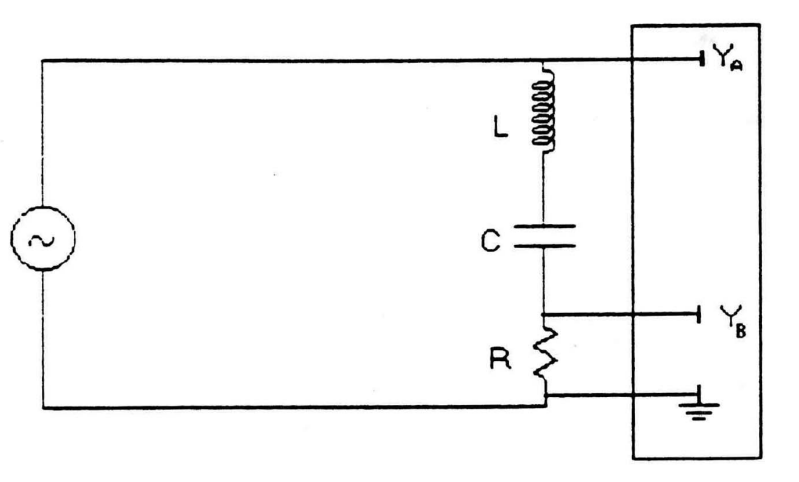
\includegraphics[width=0.5\linewidth]{screenshot005}
	\caption{Esquema del circuit usat pel règim permanent.}
	\label{fig:3.2}
\end{figure}

Variem la freqüència de la font fins que els dos senyals a l'oscil·loscopi estan en fase (usant el model DUAL del darrer). Aquesta freqüència es correspon amb la freqüència de ressonància. La comparem amb la freqüència de ressonància teòrica (en Hz)
\begin{equation}
	f_0 = \frac{1}{2\pi}\sqrt{\frac{1}{LC}},
\end{equation}
i mesurem el el guany $\abs{T_R(\omega_0)}$ corresponent a aquesta freqüència.

Mesurem les dues freqüències de tall $f_1$ i $f_2$ (en Hz)\footnote{Recordem que són les freqüències tals que $\abs{T_R(\omega_c)} = \frac{1}{\sqrt{2}}$.}. Comparem els valors mesurats amb els valors teòrics (a partir de la resolució del sistema d'equacions donat per \eqref{eq:3.38} i \eqref{eq:3.39}). Repetim tot el procediment canviant la resistència per una de $R = 270$ $\Omega$.

\subsection{Estudi del règim transitori}
Muntem el circuit de la figura \ref{fig:3.3}. Usem una bobina de $L = 33$ mH, un condensador de $C = 330$ pF, una font que ens subministri una senyal tipus \eqref{eq:3.20} i una resistència de $R = 180$ $\Omega$.

\begin{figure}[h]
	\centering
	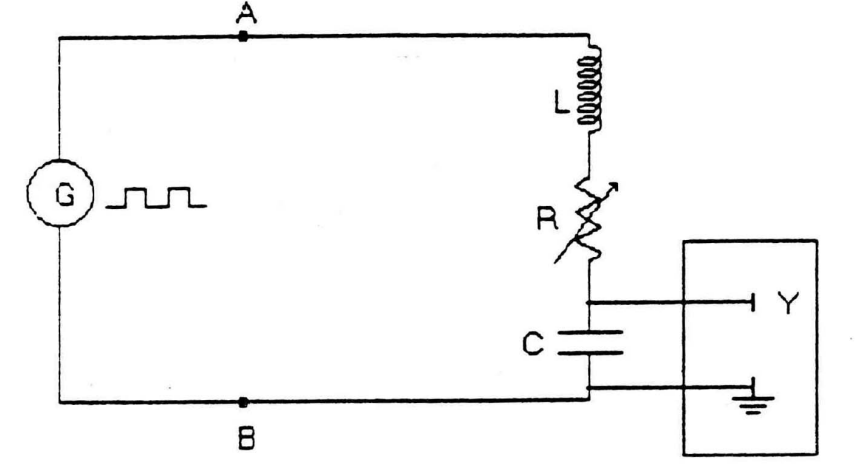
\includegraphics[width=0.5\linewidth]{screenshot006}
	\caption{Esquem del circuit usat pel règim transitori.}
	\label{fig:3.3}
\end{figure}

Fixem la freqüència del generador de forma que a cada període d'aquest, $T_{generador}$, apareguin 10 oscil·lacions de període $T$ ($f = \frac{T}{10}$), essent aquest període $T$ el corresponent a la freqüència de pseudo-pulsació, calculat usant l'equació \eqref{eq:3.25} i que
\begin{equation}
	T = \frac{2\pi}{\omega}.
\end{equation}
Seguidament mesurem el període $T$ amb l'oscil·loscopi. 

Canviem la resistència fixa per una de variable, que pot donar resistències de 0 a 100 k$\Omega$. Estudiem els casos $R<R_c$, $R=R_c$ i $R>R_c$ (on $R_c$ és la resistència crítica, donada per l'equació \eqref{eq:3.31}), de forma que podem veure les 3 solucions per a l'EDO del circuit RLC en règim transitori. Finalment, amb els valors recollits de $V_C$ i de $t$, calculem, via l'equació \eqref{eq:3.28}, el valor de la constant d'esmorteïment $\lambda$.
\section{Resultats i discussió}
posar valors teòrics i explicar d'on surten\\
\textcolor{red}{$AAAAAAAAAAAAAAAAAAAAAAAAAAAAAAAA$}
Els recull de mesures experimentals es troben a l'anex \textcolor{red}{poner anexo}. 
\subsection{Règim permanent}
Una vegada muntat el circuit de la figura \ref{fig:3.2} amb $R$, $L$ i $C$ de $2660\Omega$, $22mH$ i $15nF$ respectivament, i una font amb un voltatge d'entrada tipus $V_E = E\sin(\omega t)$, la frequència de ressonancia experimental que vam meusrar és de: \\
\begin{equation}
	f_0^{exp} = (8960 \pm 1)s^{-1}
\end{equation}\\
La qual podem comparar amb la toerica, que pel notre circuit es de:
\begin{equation}
	f_0^{teo} = \frac{1}{2\pi}\sqrt{\frac{1}{LC}} = \frac{1}{2\pi}\sqrt{\frac{1}{22 \times 10^{-3}*15 \times 10^{-9}}} = 8761 s^{-1}
\end{equation}
Com podem veure els valors son els mateixos, com calia esperar. D'altre banda, al fer la mateixa mesura pero canviant la resistencia per una de $R=274\Omega$, tot i que teoricament el valor de $f_0^{teo}$ no canvia, experiemtnalment no va ser aixi ja que vam obtenir una frequcuencia de:
\begin{equation}
	f_0^{exp} = (8860 \pm 1)s^{-1}
\end{equation}
\textcolor{red}{esto es así?? tiene sentido, o cabe la posibilidad que lo hayamos puesto mal y que realmente sea 8960 como antes...es que vaya coincidencia que solo cambie en 100 unidades no?}\\
Per comprovar si realment estem a la frequència de resonància del sistema podem calcular el guany $\abs{T_R(\omega_0)}$, que teoricmament hauria de ser $\abs{T_R^{teo}(\omega_0)} = 1$, i experimentalment:
\begin{eqnarray}
	\text{Per $R=2660\Omega$} \hspace{0.5cm} \abs{T_R^{exp}(\omega_0)} = 1 \pm 0,008\\
	\text{Per $R=274\Omega$} \hspace{0.5cm} \abs{T_R^{exp}(\omega_0)} = 0,877 \pm 0,006
\end{eqnarray}
\textcolor{red}{pues no entiendo pq cambia si estamos en la frecuencia de resonancia}\\
\\
L'altre concepte interesant del circuit RLC es mesurar les seves frequencies de tall i amb elles el seu ample de banda. Si resolem el sistema d'equacions donat per les equacions \eqref{eq:3.38} i \eqref{eq:3.39}, tenim que:
\begin{eqnarray}
	f_1^{teo} = \frac{1}{4\pi}(-\frac{R}{L} + \sqrt{(\frac{R}{L})^2 + 4\frac{1}{LC}})\\
	f_2^{teo} = \frac{R}{f_1^{teo}}\\
	\Delta \omega = \frac{R}{L}
\end{eqnarray}
Sustituint els valors de $R$, $L$, i $C$ per a les dues resistencies tenim que:\\
Per $R = 2660\Omega$:\\
\begin{center}
	\begin{tabular}{|c|c|c|c|}
		\hline
		& $f_1$ & $f_2$ & $\Delta \omega$ \\ \hline
		Teóric & $(3391 \pm 94)s^{-1}$ & $(22634 \pm 630)s^{-1}$ & $(120909 \pm 7)s^{-1}$\\ \hline
		Experimental & $(2860 \pm 1)s^{-1}$ & $(23460 \pm 1)s^{-1}$ & $(129433 \pm 9)s^{-1}$\\ \hline
	\end{tabular}
\end{center}
I per $R = 274\Omega$:
\begin{center}
	\begin{tabular}{|c|c|c|c|}
		\hline
		& $f_1$ & $f_2$ & $\Delta \omega$ \\ \hline
		Teóric & $(7826 \pm 32)s^{-1}$ & $(9808 \pm 4,0)s^{-1}$ & $(12455 \pm 10)s^{-1}$\\ \hline
		Experimental & $(8040 \pm 1)s^{-1}$ & $(9830 \pm 1)s^{-1}$ & $(11247 \pm 8)s^{-1}$\\ \hline
	\end{tabular}
\end{center}
\textcolor{red}{la table podria ser mas bonita, mirar en otro momento}
\subsection{Règim transitori}
Una vegada muntat el cricuit de la figura \ref{fig:3.3} amb $R$, $L$ i $C$ de $184\Omega$, $33mH$ i $330pF$ respectivament podem presentar els resultats. 

\textcolor{red}{$AAAAAAAAAAAAAAAAAAAAAAAAAAAAAAAA$}
\section{Conclusions}


\chapter{Inductància mútua i transformadors}

\begin{chapterabstract}
	\textit{Vejam, digué el cec.}
\end{chapterabstract}

\section{Introducció i fonament teòric}
El 1831, Faraday va realitzar un experiment que va permetre comprovar que, en variar el flux que travessa la superfície d'un circuit tancat, en aquest s'hi genera un corrent que l'anomenarem induït.

Aquest fenomen pot ser descrit de la següent manera:
\begin{equation}
	\oint_c \Vec{E}\cdot \mathrm{d}\Vec{l}_c = -\dv{}{t} \int \Vec{B}\cdot \mathrm{d} \Vec{S}_c = - \dv{\Phi}{t} \label{eq:4:1}
\end{equation}
Veiem que la integral és tancada sobre una línia $C$ que delimita la superfície $S_c$, la qual experimenta una variació de flux magnètic $\Phi$ en el temps.

L'expressió anterior té unitats de volts però, tot i així, aquesta integral es designa com la \textit{força electromotriu induïda}.

Aquesta força dividida entre la resistència del circuit considerat és igual al corrent que s'induiria en el cas de tenir una bateria d'aquest mateix voltatge i polaritat.

El camp d'inducció magnètica $\Vec{B}$ i la intensitat $I$ que l'indueix són, per a qualsevol punt que considerem, proporcionals entre si. Per tant, es conclou que també ho serà $\Phi$, de manera que:
\begin{equation}
	\Phi=LI \label{eq:4:2}
\end{equation}
Aquí hem introduït l'\textit{autoinductància} o \textit{autoinducció del circuit}, una constant que depèn de la geometria del circuit i de la permeabilitat del medi d'immersió. És clar que, per l'equació \eqref{eq:4:2}, la $L$ tindrà unitats de weber per amper, és a dir, henrys (H).

Considerem ara un parell de circuits o bobines situades prop una de l'altra. Si per la primera hi circula un corrent $I_1$, conseqüentment travessarà per la segona un flux $\Phi_2$. Com que aquestes dues magnituds han de ser proporcionals,
\begin{equation}
	\Phi_2=M_{12}I_2 \label{eq:4:3}
\end{equation}
on $M_{21}$ és la \textit{inductància mútua} entre circuits i també es mesura en henrys.

De manera anàloga al que passava amb la primera bobina que induïa un corrent a la segona, el cas invers també es donarà. Per tant, pel circuit 1 travessarà un flux $\Phi_1$ causat pel corrent de la bobina 2, de manera que
\begin{equation}
	\Phi_1=M_{12}I_2 \label{eq:4:4}
\end{equation}
Per definició, sabem que
\begin{equation}
	\Phi_2=\int_{S_2}\vec{B}_1 \cdot \mathrm{d}\Vec{S}_2 \label{eq:4:5}
\end{equation}
Amb totes aquestes equacions mencionades fins ara, es demostra fàcilment l'equació de Neumann:
\begin{equation}
	M_{ab}=\frac{\mu_0}{4\pi}\oint_a\oint_b\frac{\mathrm{d}\Vec{l}_a\cdot\mathrm{d}\Vec{l}_b}{r} \label{eq:4:6}
\end{equation}
Aquesta equació és simètrica respecte $a$ i $b$, és a dir
\begin{equation}
	M_{12}=M_{21}. \label{eq:4:7}
\end{equation}
Un transformador consisteix en un parell de bobines amb un nucli d'un material de molt alta permeabilitat (aleacions de ferro amb un petit percentatge de silici o altres aliatges més barats) que concentra les línies de camp magnètic, evitant així la disminució de flux. A més, per tal de minimitzar les pèrdues de potència causades pels corrents de Foucault que s'indueixen aplicant un corrent altern, el nucli es constitueix d'un seguit de làmines aïllades unes de les altres. 

Així, depenent dels paràmetres escollits pel transformador, en aplicar un corrent altern a una d'elles, el voltatge mesurat a la sortida de la segona tindrà un valor diferent.

El funcionament d'una bobina, però, es pot simplificar molt considerant que les dues bobines es troben enrotllades de tal manera que el flux que genera una d'elles passarà per la segona (i anàlogament amb el cas invers). Amb aquesta configuració, es compleix que
\begin{equation}
	\frac{\Phi_1}{\Phi_2}=\frac{L_1I_1}{MI_1}=\frac{L_1}{M}=\frac{n_1}{n_2}, \label{eq:4:8}
\end{equation}
on denotem amb una $M$ la inductància mútua entre bobines, ja que $M_{12}=M_{21}$. Per altra banda, $n_1$ i $n_2$ són el nombre de voltes de les bobines 1 i 2, respectivament.

Naturalment, pel cas invers tindrem
\begin{equation}
	\frac{\Phi_2}{\Phi_1}=\frac{L_2I_2}{MI_2}=\frac{L_2}{M}=\frac{n_2}{n_1}, \label{eq:4:9}
\end{equation}
de manera que
\begin{equation}
	M^2=L_1L_2. \label{eq:4:10}
\end{equation}
Treballant en fluxos que travessen les bobines, si aquests varien amb el temps, la relació entre els voltatges que s'induiran serà la divisió entre el nombre de voltes de la primera bobina entre les voltes de la segona. Per tant:
\begin{equation}
	\frac{V_1}{V_2}=\frac{\dv{\Phi_1}{t}}{\dv{\Phi_2}{t}}=\frac{n_1}{n_2}. \label{eq4:11}
\end{equation}
En termes de nomenclatura, anomenarem \textit{primari} al voltatge d'entrada $V_1$ i \textit{secundari} al de sortida $V_2$.

Tot el descrit fins ara fa referència a un cas ideal però el que s'observa experimentalment és que $M$ és menor a l'esperat, ja que no tot el flux del primer circuit entra a l'altre. Per això, hem d'introduir un paràmetre $k$ denominat coeficient d'acoblament, tal que
\begin{equation}
	M=k(L_1L_2)^{1/2}.
\end{equation}
És notori, doncs, que el coeficient $k$ prendrà valors entre 0 i 1, sent aquest últim el cas ideal.

\section{Metodologia experimental}

\section{Resultats i discussió}

\section{Conclusions}

\chapter{Mesura de la resistència d'un metall}

\begin{chapterabstract}
	\textit{Here goes blahblahblah$\ldots$}
\end{chapterabstract}

\section{Introducció i fonament teòric}

\section{Metodologia experimental}

\section{Resultats i discussió}

\section{Conclusions}


\begin{thebibliography}{99}
	\bibitem{ref1}
	\textit{Col·lecció de problemes de l'assignatura d'Electromagnetisme.}
\end{thebibliography}

\newpage
\begin{appendices}
%SI TOQUEU AIXÒ ELS ANNEXOS PETEN.

\textbf{\Huge{Annexos}}
\renewcommand{\thesection}{\Alph{section}} % Cambia la numeración de capítulos a letras
\renewcommand{\theequation}{\thesection.\arabic{equation}} % Cambia numeración de ecuaciones
\setcounter{equation}{0} % Reinicia contador de ecuaciones en cada sección

\section{Càlcul d'incerteses}
\label{an:a3}
Pel càlcul de les incerteses associades a cada pràctica s'ha utilitzat la llei de propagació d'incerteses:
\begin{equation}
	u_F = \sqrt{ \left( \frac{\partial F}{\partial x_1} \right)^2 u_{x_1}^2 + \left( \frac{\partial F}{\partial x_2} \right)^2 u_{x_2}^2 + \dots + \left( \frac{\partial F}{\partial x_n} \right)^2 u_{x_n}^2 },
\end{equation}
on $F(x_1,x_2,\ldots,x_n)$ és la funció considerada i $u_i$ la incertesa associada a cada $x_i$.

\subsection{Incerteses pràctica 1}
Per simplicitat anomenem $\frac{\Delta V_i \Delta l_i}{\Delta r_i} = Y_i$, de forma que:
\begin{equation}
	u_{Y_i} = \sqrt{ \left( \frac{\Delta l_i \Delta V_i}{\Delta r_i} u_{\Delta V_i} \right)^2 + \left( \frac{\Delta V_i \Delta l_i}{\Delta r_i} u_{\Delta l_i} \right)^2 + \left( \frac{\Delta l_i \Delta V_i}{\Delta r_i^2} u_{\Delta r_i} \right)^2 },
\end{equation}
\begin{equation}
	\frac{Q}{Z} = \varepsilon \sum_i Y_i \implies u_{Q/Z} = \varepsilon \sqrt{\sum_i u_{Y_i}^2},
\end{equation}
\begin{equation}
	u_{\frac{C}{Z}} = \sqrt{ \left( \frac{1}{Z \, \Delta V} u_Q \right)^2 + \left( \frac{Q}{Z \, \Delta V^2} u_{\Delta V} \right)^2 },
\end{equation}
\begin{equation}
	u_{C_\text{teòric}} = \frac{u_H}{d} \sqrt{1+C^2}.
\end{equation}


\newpage
\section{Annex pràctica 1. Representació de camps}
\subsection{Deducció de l'equació $(1.22)$}
\label{an:a1}
Per deduir l'expressió donada per l'equació \eqref{eqsuppon} ens basarem ens els resultats del problema 2.18 de la llista de problemes de l'assignatura \cite{ref1}. Suposem dos fils infinits rectilinis i carregats amb densitat de càrrega uniforme $\lambda$ i -$\lambda$ separats per una distància $d=2a$. Siguin $\rho_1$ i $\rho_2$ les distàncies radials de cada fil al punt en el qual volem calcular el camp i el potencial. Per la simetria del sistema podem assegurar que $\vec{E}(\vec{r}) = E(\rho) \vec{e}_{\rho}$, de forma que podem aplicar el teorema de Gauss com se segueix:

\[
\left.
\begin{array}{c}
	\oint \vec{E} \cdot \mathrm{d}\vec{S} = E 2\pi \rho L \\[10pt]
	\frac{Q_{int}}{\varepsilon_0} = \frac{1}{\varepsilon_0} \int \lambda \, \mathrm{d}l = \frac{\lambda}{\varepsilon_0} L
\end{array}
\right\}
\quad \Rightarrow \quad 
\vec{E} = \frac{\lambda}{2\pi \varepsilon_0} \frac{1}{\rho} \vec{e}_{\rho}.
\]

Així, essent $\vec{E_1}$ el camp associat al fil amb densitat $\lambda$ i $\vec{E_2}$ el camp associat al fil amb densitat -$\lambda$, tenim:
\begin{align}
	\vec{E_1} & = \frac{\lambda}{2\pi \varepsilon_0} \frac{1}{\rho_1} \vec{e}_{\rho_1}, \\
	\vec{E_2} & = -\frac{\lambda}{2\pi \varepsilon_0} \frac{1}{\rho_2} \hat{e}_{\rho_2},
\end{align}
on:
\begin{align}
	\rho_1 & = \sqrt{(x-a)^2+y^2}, \\
	\rho_2 & = \sqrt{(x+a)^2+y^2}. 
\end{align}
Si calculem el camp usant que
\begin{equation}
	\phi(r) = -\int_{\vec{r}_{ref}}^{\vec{r}}\vec{E}(\vec{r})\cdot \mathrm{d}\vec{r} ,
\end{equation}
i aplicant el principi de superposició, és a dir
\begin{equation}
	\phi = \phi_1+\phi_2,
\end{equation}
trobem que, el potencial generat per aquesta distribució de càrrega obeeix la següent equació:
\begin{equation}
	\phi = \frac{\lambda}{2\pi \varepsilon_0}\ln\sqrt{\frac{(x+a)^2+y^2}{(x-a)^2+y^2}}.
\end{equation}
Les superfícies equipotencials seran aquelles regions de l'espai en què el potencial sigui constant. Escollint
\begin{equation}
	k \equiv e^{\frac{\phi2\pi\varepsilon_0}{\lambda}} = \sqrt{\frac{(x+a)^2+y^2}{(x-a)^2+y^2}},
\end{equation}
i reescrivint segons
\begin{equation}
	k^2[(x-a)^2+y^2]=(x+a)^2+y^2,
\end{equation}  
podem desenvolupar fins a arribar a
\begin{equation}
	\boxed{y^2+\left( x+a\frac{1+k^2}{1-k^2}\right)^2 = a^2\left( \frac{2k}{1-k^2}\right)^2},
\end{equation}
que és l'equació per les superfícies (línies) equipotencials.

\newpage
\subsection{Expressió analítica de la distribució de dos plans secants i un fil}
\label{an:a6}
Per obtenir les expressions analítiques apliquem la definició del potencial i integrem
\begin{equation}
	\phi (x,y) = \frac{1}{4\pi\varepsilon}\int_S\frac{\sigma(x',y')}{\sqrt{(x-x')^2+(y-y')^2}}\mathrm{d}s'.
\end{equation}
Les coordenades prima son les referents a la distribució de carrega i $S$ tota la regió on hi hagi càrrega. Separarem la distribució en tres parts: la càrrega puntual, la part de la placa inferior i la superior, finalment apliquem el principi de superposició per conèixer el potencial que crea la nostra distribució. El potencial que crea la càrrega puntual a la posició $\vec{r_q}$ és:
\begin{equation}
	\phi_q (x,y) = -\frac{1}{4\pi\varepsilon}\frac{q}{\sqrt{(x-d)^2+y^2}}.
\end{equation}
Per resoldre la integral per les plaques hem de tenir en compte que és una distribució unidimensional de càrrega, de manera que $\sigma(x',y') \rightarrow \lambda(x',y')$ i $\mathrm{d}s' \rightarrow \mathrm{d}L$. Per la geometria del problema podem veure que $y' = \tan(\pi/6)x'$ per la placa superior i $y' = -\tan(\pi/6)x'$ per la inferior, de forma que $\phi_{sup}(x,y) = \phi_{inf}(x,-y)$. Per tant:
\begin{align}
	\phi_{sup}(x,y)&=\frac{1}{4\pi\varepsilon}\int_{0}^{\frac{\sqrt{3}}{2}L} \frac{q/L}{\sqrt{(x-x')^2+(y-\frac{\sqrt{3}}{2}x')^2}}\mathrm{d}x', \\
	\phi_{sup}(x,y)&=\frac{1}{4\pi\varepsilon}\frac{\sqrt{3}}{2}\ln \left[\frac{\frac{4}{\sqrt{3}}\sqrt{(x^2+y^2)+L(-\sqrt{3}x+y+L)}+\frac{2}{3}(-3x+\sqrt{3}y+2\sqrt{3}L)}{\frac{4}{\sqrt{3}}\sqrt{x^2+y^2}-\frac{2}{3}(3x-\sqrt{3}y)}\right].
\end{align}
Finalment, podem trobar el potencial total segons:
\begin{equation}
	\phi(x,y) = \phi_q(x,y) + \phi_{sup}(x,y) + \phi_{sup}(x,-y). \\
\end{equation}
El camp elèctric, per la seva banda, serà:
\begin{equation}
	\vec{E}(x,y) = -\vec{\nabla}\phi(x,y).
\end{equation}
\newpage
\subsection{Dades experimentals de la pràctica 1}
\label{an:a2}
A continuació mostrem els valors experimentals obtinguts en el transcurs de la pràctica 1.
\begin{table}[h]
	\centering
	\renewcommand{\arraystretch}{1.2}
	\caption{Taula amb els valors experimentals mesurats per tal de poder calcular la capacitat del condensador de plaques planoparal·leles.}
	\begin{tabular}{cccc}
		\toprule
		$\Delta l_i$ (m) & $\Delta r_i$ (m) & $\Delta V_i$ (V) & $\frac{\Delta V_i\Delta l_i}{\Delta r_i}$ (V)\\
		\midrule
		0.005 $\pm$ 0.001 & 0.019 $\pm$ 0.001 & 1.00 $\pm$ 0.01 & 0.26 $\pm$ 0.23 \\
		0.005 $\pm$ 0.001 & 0.024 $\pm$ 0.001 & 1.00 $\pm$ 0.01 & 0.21 $\pm$ 0.20 \\
		0.010 $\pm$ 0.001 & 0.038 $\pm$ 0.001 & 1.00 $\pm$ 0.01 & 0.26 $\pm$ 0.16 \\
		0.010 $\pm$ 0.001 & 0.050 $\pm$ 0.001 & 1.00 $\pm$ 0.01 & 0.20 $\pm$ 0.14 \\
		0.005 $\pm$ 0.001 & 0.057 $\pm$ 0.001 & 1.00 $\pm$ 0.01 & 0.09 $\pm$ 0.13 \\
		0.005 $\pm$ 0.001 & 0.063 $\pm$ 0.001 & 1.00 $\pm$ 0.01 & 0.08 $\pm$ 0.13 \\
		0.010 $\pm$ 0.001 & 0.070 $\pm$ 0.001 & 1.00 $\pm$ 0.01 & 0.14 $\pm$ 0.12 \\
		0.005 $\pm$ 0.001 & 0.071 $\pm$ 0.001 & 1.00 $\pm$ 0.01 & 0.07 $\pm$ 0.12 \\
		0.009 $\pm$ 0.001 & 0.066 $\pm$ 0.001 & 1.00 $\pm$ 0.01 & 0.14 $\pm$ 0.12 \\
		0.010 $\pm$ 0.001 & 0.034 $\pm$ 0.001 & 1.00 $\pm$ 0.01 & 0.29 $\pm$ 0.17 \\
		0.008 $\pm$ 0.001 & 0.024 $\pm$ 0.001 & 1.00 $\pm$ 0.01 & 0.33 $\pm$ 0.20 \\
		0.005 $\pm$ 0.001 & 0.014 $\pm$ 0.001 & 1.00 $\pm$ 0.01 & 0.36 $\pm$ 0.27 \\
		0.005 $\pm$ 0.001 & 0.009 $\pm$ 0.001 & 1.00 $\pm$ 0.01 & 0.56 $\pm$ 0.34 \\
		0.002 $\pm$ 0.001 & 0.004 $\pm$ 0.001 & 1.00 $\pm$ 0.01 & 0.50 $\pm$ 0.52 \\
		0.002 $\pm$ 0.001 & 0.003 $\pm$ 0.001 & 1.00 $\pm$ 0.01 & 0.67 $\pm$ 0.62 \\
		0.003 $\pm$ 0.001 & 0.004 $\pm$ 0.001 & 1.00 $\pm$ 0.01 & 0.75 $\pm$ 0.53 \\
		0.010 $\pm$ 0.001 & 0.005 $\pm$ 0.001 & 1.00 $\pm$ 0.01 & 2.00 $\pm$ 0.60 \\
		0.010 $\pm$ 0.001 & 0.006 $\pm$ 0.001 & 1.00 $\pm$ 0.01 & 1.67 $\pm$ 0.49 \\
		0.010 $\pm$ 0.001 & 0.006 $\pm$ 0.001 & 1.00 $\pm$ 0.01 & 1.67 $\pm$ 0.49 \\
		0.010 $\pm$ 0.001 & 0.006 $\pm$ 0.001 & 1.00 $\pm$ 0.01 & 1.67 $\pm$ 0.49 \\
		0.010 $\pm$ 0.001 & 0.005 $\pm$ 0.001 & 1.00 $\pm$ 0.01 & 2.00 $\pm$ 0.60 \\
		0.010 $\pm$ 0.001 & 0.005 $\pm$ 0.001 & 1.00 $\pm$ 0.01 & 2.00 $\pm$ 0.60 \\
		0.010 $\pm$ 0.001 & 0.006 $\pm$ 0.001 & 1.00 $\pm$ 0.01 & 1.67 $\pm$ 0.49 \\
		0.005 $\pm$ 0.001 & 0.005 $\pm$ 0.001 & 1.00 $\pm$ 0.01 & 1.00 $\pm$ 0.49 \\
		0.002 $\pm$ 0.001 & 0.005 $\pm$ 0.001 & 1.00 $\pm$ 0.01 & 0.40 $\pm$ 0.45 \\
		0.002 $\pm$ 0.001 & 0.006 $\pm$ 0.001 & 1.00 $\pm$ 0.01 & 0.33 $\pm$ 0.41 \\
		0.003 $\pm$ 0.001 & 0.007 $\pm$ 0.001 & 1.00 $\pm$ 0.01 & 0.43 $\pm$ 0.38 \\
		0.005 $\pm$ 0.001 & 0.011 $\pm$ 0.001 & 1.00 $\pm$ 0.01 & 0.45 $\pm$ 0.30 \\
		\bottomrule
	\end{tabular}
	\label{tab:valores}
\end{table}

Amb aquests valors i usant l'equació \eqref{eq1.17} podem determinar la capacitat del condensador de plaques planoparal·leles dibuixat.

\newpage
\subsection{Codis de les simulacions de la pràctica 1}
\label{an:a4}
Tot seguit adjuntem els diferents codis usats per generar les simulacions dels camps i les corbes equipotencials usant Python:.

El codi per la simulació del condensador de plaques planoparal·leles és:
\begin{lstlisting}
import numpy as np
import matplotlib.pyplot as plt

# Definim el camp electric 
def E(q, r0, x, y):
rx, ry = x - r0[0], y - r0[1]
dist = (rx**2 + ry**2)**1.5
return q * rx / dist, q * ry / dist

# Definim el potencial electric
def V(q, r0, x, y):
return q / np.hypot(x - r0[0], y - r0[1])

# Malla
x = np.linspace(-6, 6, 100)
y = np.linspace(-5, 5, 100)
X, Y = np.meshgrid(x, y)

q1, q2 = 1, -1
d = 4
charges = [(q1, (d/2, 0)), (q2, (-d/2, 0))]

Ex, Ey = np.zeros(X.shape), np.zeros(Y.shape)
Vt = np.zeros(X.shape)
for q, pos in charges:
ex, ey = E(q, pos, X, Y)
Ex += ex
Ey += ey
Vt += V(q, pos, X, Y)

fig, ax = plt.subplots()
ax.streamplot(X, Y, Ex, Ey, color=np.log(np.hypot(Ex, Ey)), linewidth=0.7, cmap=plt.cm.plasma, density=1)
ax.contour(X, Y, Vt, levels=np.linspace(-2, 2, 20), colors='black', linestyles='solid', linewidths=0.5)

for q, pos in charges:
color = 'red' if q < 0 else 'blue'
ax.scatter(*pos, color=color, s=100)

ax.set_aspect('equal')
ax.set_xticks([])
ax.set_yticks([])
ax.spines['top'].set_visible(True)
ax.spines['right'].set_visible(True)
ax.spines['left'].set_visible(True)
ax.spines['bottom'].set_visible(True)
plt.show()
\end{lstlisting}

El codi per la simulació dels dos fils infinits és:
\begin{lstlisting}
import numpy as np
import matplotlib.pyplot as plt

# Definim el camp electric
def E(q, r0, x, y):
    rx, ry = x - r0[0], y - r0[1]
    dist = (rx**2 + ry**2)**1.5
    return q * rx / dist, q * ry / dist

# Definim el potencial electric
def V(q, r0, x, y):
    return q / np.hypot(x - r0[0], y - r0[1])

# Malla
x = np.linspace(-6, 6, 100)
y = np.linspace(-5, 5, 100)
X, Y = np.meshgrid(x, y)

q1, q2 = 1, -1
d = 4
charges = [(q1, (d/2, 0)), (q2, (-d/2, 0))]

Ex, Ey = np.zeros(X.shape), np.zeros(Y.shape)
Vt = np.zeros(X.shape)
for q, pos in charges:
    ex, ey = E(q, pos, X, Y)
    Ex += ex
    Ey += ey
    Vt += V(q, pos, X, Y)

fig, ax = plt.subplots()
ax.streamplot(X, Y, Ex, Ey, color=np.log(np.hypot(Ex, Ey)), linewidth=0.7, cmap=plt.cm.plasma, density=1)
ax.contour(X, Y, Vt, levels=np.linspace(-2, 2, 20), colors='black', linestyles='solid', linewidths=0.5)

for q, pos in charges:
    color = 'red' if q < 0 else 'blue'
    ax.scatter(*pos, color=color, s=100)

ax.set_aspect('equal')
ax.set_xticks([])
ax.set_yticks([])
ax.spines['top'].set_visible(True)
ax.spines['right'].set_visible(True)
ax.spines['left'].set_visible(True)
ax.spines['bottom'].set_visible(True)
plt.show()
\end{lstlisting}

El codi per la simulació dels dos plans secants i el fil infinit pel mètode de les càrregues imatge és:
\begin{lstlisting}
import numpy as np
import matplotlib.pyplot as plt
from matplotlib import colormaps
import sympy as sp
import latexify

q = 1
d= 4.603
nx, ny = 128, 128
L = (10.019+10.610)/2

#cosas de los graficos
x = np.linspace(-2.5, 13, 1500) #-1.5 / 4.2 / 50
y = np.linspace(-7, 7, 1500) #-2.5 / 2.5 / 50
X, Y = np.meshgrid(x, y)



#func potencaial
def V(x,y):
return -q*(1/np.sqrt((x-d)**2+(y)**2) - 1/np.sqrt((x-d/2)**2+(y-d*np.sqrt(3)/2)**2) +1/np.sqrt((x+d/2)**2+(y-d*np.sqrt(3)/2)**2) -1/np.sqrt((x+d)**2+(y)**2) +1/np.sqrt((x+d/2)**2+(y+d*np.sqrt(3)/2)**2) -1/np.sqrt((x-d/2)**2+(y+d*np.sqrt(3)/2)**2))

Z = V(X, Y)

def E_x(x,y):
return -(q*((x-d)/(np.sqrt((x-d)**2+(y)**2))**(3/2) - (x-d/2)/(np.sqrt((x-d/2)**2+(y-d*np.sqrt(3)/2)**2))**(3/2) +(x+d/2)/(np.sqrt((x+d/2)**2+(y-d*np.sqrt(3)/2)**2))**(3/2) -(x+d)/(np.sqrt((x+d)**2+(y)**2))**(3/2) +(x+d/2)/(np.sqrt((x+d/2)**2+(y+d*np.sqrt(3)/2)**2))**(3/2) -(x-d/2)/(np.sqrt((x-d/2)**2+(y+d*np.sqrt(3)/2)**2))**(3/2)))

def E_y(x,y):
return -(q*((y)/(np.sqrt((x-d)**2+(y)**2))**(3/2) - (y-d*np.sqrt(3)/2)/(np.sqrt((x-d/2)**2+(y-d*np.sqrt(3)/2)**2))**(3/2) +(y-d*np.sqrt(3)/2)/(np.sqrt((x+d/2)**2+(y-d*np.sqrt(3)/2)**2))**(3/2) -(y)/(np.sqrt((x+d)**2+(y)**2))**(3/2) +(y+d*np.sqrt(3)/2)/(np.sqrt((x+d/2)**2+(y+d*np.sqrt(3)/2)**2))**(3/2) -(y+d*np.sqrt(3)/2)/(np.sqrt((x-d/2)**2+(y+d*np.sqrt(3)/2)**2))**(3/2)))

E_xx = E_x(X,Y)
E_yy = E_y(X,Y)

#el plot
fig =plt.figure(figsize=(10.714, 9.286), label= 'Linies de camp') 
ax = fig.add_subplot(111)

ax.contour(X,Y,Z, levels =np.linspace(-3, 3, 30), colors='black',linewidths=0.5, linestyles='solid')
ax.streamplot(X,Y,E_xx,E_yy, density=2.5, color=np.log(np.hypot(E_xx, E_yy)), cmap='plasma', linewidth=0.5)
#plt.contourf(X, Y, normP, cmap="rainbow", levels=60)
#plt.contourf(X, Y, normPM, cmap="rainbow", levels=60)


#puntos de las cargas
#pa = np.linspace(0,L*np.sqrt(3)/2, 2000)

ax.plot([d],[0], 'bo', markersize=14)
ax.plot([d/2],[d*np.sqrt(3)/2], 'ro', markersize=14)
ax.plot([-d/2],[d*np.sqrt(3)/2], 'bo', markersize=14)
ax.plot([-d/2],[-d*np.sqrt(3)/2], 'bo', markersize=14)
ax.plot([d/2],[-d*np.sqrt(3)/2], 'ro', markersize=14)

#ax.plot([pa],[np.sqrt(3)/3*pa],'ro', markersize=3)
#configs del grafico
ax.set_xticks([])
ax.set_yticks([])
ax.set_aspect('equal')
plt.show()
\end{lstlisting}

El codi per la simulació analítica dels dos plans secants i el fil infinit és:
\begin{lstlisting}
import numpy as np
import matplotlib.pyplot as plt
from matplotlib import colormaps
import sympy as sp
import latexify



L = (10.019+10.610)/2
q =1
d = 4.603
u = (q/L)*np.sqrt(3)/2

def f(x, y):
a = 4/np.sqrt(3)
b = a*np.sqrt(x**2+y**2)-(2/3)*(3*x-np.sqrt(3)*y)
p = 1/np.sqrt((x-d)**2+y**2)
return u*np.log(((a*np.sqrt((x**2+y**2)+L*(-np.sqrt(3)*x-y+L))+2/3*(-3*x-np.sqrt(3)*y+2*np.sqrt(3)*L)))/(a*np.sqrt(x**2+y**2)-(2/3)*(3*x+np.sqrt(3)*y)))+u*np.log((a*np.sqrt((x**2+y**2)+L*(-np.sqrt(3)*x+y+L))+2/3*(-3*x+np.sqrt(3)*y+2*np.sqrt(3)*L))/b)-q*p

x = np.linspace(-2.5, 13, 1500) #-1.5 / 4.2 / 50
y = np.linspace(-7, 7, 1500) #-2.5 / 2.5 / 50
X, Y = np.meshgrid(x, y)
Z = f(X, Y)


def F(x,y):
return 4/np.sqrt(3)*np.sqrt(x**2+y**2+L*(y-np.sqrt(3)*x+L))+2/3*(np.sqrt(3)*y-3*x+2*np.sqrt(3)*L)

def F_x(x,y):
return 2/np.sqrt(3)*(2*x-np.sqrt(3)*L)/(np.sqrt(x**2+y**2+L*(y-np.sqrt(3)*x+L)))-2

def F_y(x,y):
return 2/np.sqrt(3)*(2*y+L)/(np.sqrt(x**2+y**2+L*(y-np.sqrt(3)*x+L)))+2/np.sqrt(3)


def V(x,y):
return 4/np.sqrt(3)*np.sqrt(x**2+y**2)+2/3*(np.sqrt(3)*y-3*x)

def V_x(x,y):
return 4/np.sqrt(3)*x/(np.sqrt(x**2+y**2))-2

def V_y(x,y):
return 4/np.sqrt(3)*y/np.sqrt(x**2+y**2)+2/np.sqrt(3)


Ex = -u*(F_x(X,Y)/F(X,Y) + F_x(X,-Y)/F(X,-Y) -V_x(X,Y)/V(X,Y)-V_x(X,-Y)/V(X,-Y)) -q*(X-d)/(((X-d)**2+Y**2)**(3/2))
Ey = -u*(F_y(X,Y)/F(X,Y) - F_y(X,-Y)/F(X,-Y) -V_y(X,Y)/V(X,Y)+V_y(X,-Y)/V(X,-Y)) -q*Y/(((X-d)**2+Y**2)**(3/2))

normE = np.log(np.sqrt(Ex**2+Ey**2))
normP = np.log(-Z)
normPM = np.log(Z)

fig =plt.figure(figsize=(10.714, 9.286), label= 'Linies de camp') 
ax = fig.add_subplot(111)

ax.contour(X,Y,Z, levels =np.linspace(-3, 3, 30), colors='black',linewidths=0.5, linestyles='solid')
ax.streamplot(X,Y,Ex,Ey, density=2.5, color=np.log(np.hypot(Ex, Ey)),cmap='plasma', linewidth=0.5)
#colorin = ax.contourf(X, Y, normE, cmap="rainbow", levels=60)
#plt.contourf(X, Y, normP, cmap="rainbow", levels=60)
#plt.contourf(X, Y, normPM, cmap="rainbow", levels=60)
ax.set_xticks([])
ax.set_yticks([])

ax.plot([d],[0], 'bo', markersize=14)
pa = np.linspace(0,L*np.sqrt(3)/2-.01, 2000)
ax.plot([pa],[np.sqrt(3)/3*pa],'ro', markersize=3)
ax.plot([pa],[-np.sqrt(3)/3*pa],'ro', markersize=3)

plt.show()
\end{lstlisting}



\end{appendices}

\end{document}
